% !TeX program = pdflatex
\documentclass{iutbscthesis}
\usepackage{multirow}
\usepackage{tabularx}
\usepackage{array}
\addbibresource{citations.bib}

\title{Robustness and Recovery of Digital Twin-Pretrained Beam Prediction Models for O-RAN Networks Under Real-World Post-Deployment Environmental Shifts}

\addauthor{Namisa Najah Raisa}{210042112}
\addauthor{Ishmaam Iftekhar Khan}{210042125}
\addauthor{Faiza Maliat}{210042163}

\supervisor{Dr.\ Md Moniruzzaman}{Assistant Professor}{Department of Computer Science and Engineering}

\addcosupervisor{Faisal Hussain}{Assistant Professor}{Department of Computer Science and Engineering}

\department{Department of Computer Science and Engineering}

\program{BACHELOR OF SCIENCE IN COMPUTER SCIENCE AND ENGINEERING}

\defensedate{22}{April}{2026}

\begin{document}

%-------------------------- FRONT MATTER --------------------------%

\coverpage

\pagenumbering{roman}

\titlepage

\declarationofcandidate

\dedicatedto{everyone trying to make digital twins tell the truth about what they do not know}

\tableofcontents
\listoffigures
\listoftables

\clearpage

\begin{abbreviations}
    \abbr{AoD}{Angle of Departure}
    \abbr{BS}{Base Station}
    \abbr{CSI}{Channel State Information}
    \abbr{DL}{Deep Learning}
    \abbr{DT}{Digital Twin}
    \abbr{FDD}{Frequency Division Duplex}
    \abbr{GPS}{Global Positioning System}
    \abbr{LoS}{Line-of-Sight}
    \abbr{MIMO}{Multiple-Input Multiple-Output}
    \abbr{ML}{Machine Learning}
    \abbr{mmWave}{Millimeter Wave}
    \abbr{MLP}{Multi-Layer Perceptron}
    \abbr{NLoS}{Non-Line-of-Sight}
    \abbr{OFDM}{Orthogonal Frequency-Division Multiplexing}
    \abbr{RSRP}{Reference Signal Received Power}
    \abbr{RT}{Ray Tracing}
    \abbr{TL}{Transfer Learning}
    \abbr{UE}{User Equipment}
    \abbr{ULA}{Uniform Linear Array}
    \abbr{V2I}{Vehicle-to-Infrastructure}
\end{abbreviations}

\begin{acknowledgement}

We would like to express our sincere gratitude to our supervisor, Dr.\ Md Moniruzzaman, Assistant Professor, Department of Computer Science and Engineering, and our co-supervisor, Faisal Hussain, Assistant Professor, Department of Computer Science and Engineering, for their guidance, patience, and continual feedback throughout the development of this research.

We are thankful to the Islamic University of Technology and the Department of Computer Science and Engineering for the resources and environment that made this work possible.

We also acknowledge the Wireless Intelligence Lab at Arizona State University for releasing the DeepMIMO and DeepSense~6G datasets and the accompanying digital twin research that this thesis builds directly upon, and to our families for their patience and support throughout this undergraduate research journey.

\end{acknowledgement}

\begin{abstract}
Digital twins have been proposed as a way to train deep learning models for millimeter wave beam prediction without collecting large volumes of real-world channel measurements, and prior work has shown that a model pretrained on synthetic, ray-traced digital twin data can be fine-tuned to near-optimal accuracy with as few as twenty real samples at a single fixed site. What remains unexamined is what happens after such a model is deployed: the physical environment a base station serves does not stay fixed, and a digital twin built once at deployment time cannot be expected to remain valid indefinitely, or to transfer to a nearby but different physical environment, without being told so. This thesis studies the following question: how does a digital-twin-pretrained, transfer-learning-refined beam prediction model degrade when the deployment environment shifts along two realistic axes -- time-of-day and physical site -- and how efficiently can it be recovered using a small number of newly collected real-world samples? We propose a two-stage, purely measurement-driven methodology that requires no new ray tracing. Stage~0 reproduces the original digital-twin-to-real transfer learning pipeline of Jiang and Alkhateeb on DeepSense~6G Scenario~1, obtaining a zero-shot top-2 accuracy of 91.53\%, closely matching the originally published 91.4\%, and validating the pipeline before any new question is introduced. Stage~1 evaluates four controlled, single-factor real-to-real comparisons built from two matched pairs of DeepSense~6G vehicle-to-infrastructure scenarios -- two street sites, each captured in daytime and nighttime conditions -- so that the effect of a time-of-day shift and the effect of a site shift can be measured independently rather than confounded together. The results show that the two shift types are not merely different in degree but different in kind: a time-of-day shift degrades zero-shot accuracy to 1.25--3.9 times the random-chance level and recovers steadily with modest amounts of real data, whereas a site shift collapses zero-shot accuracy to as low as 3\% of random chance and remains at approximately chance level even after two hundred real fine-tuning samples. A dedicated ablation, which fixes the amount of real data and instead doubles the fine-tuning epoch budget, shows that this recovery is driven specifically by additional real data rather than by additional optimization steps, since doubling the epoch budget alone changes accuracy by less than 0.1 percentage points. These findings indicate that the sample-efficient recovery previously demonstrated for the synthetic-to-real digital twin gap does not automatically transfer to real-to-real post-deployment environmental shifts, and that the cost of recovery depends materially on which aspect of the environment has changed. To determine whether the severity of the site-shift finding is a property of the site-shift task itself or of the specific transfer-learning recipe used to recover from it, we further repeat the Stage~1 protocol on three additional, substantially cheaper non-parametric models: k-nearest neighbors, random forest, and a Fourier-feature-augmented variant of k-nearest neighbors. Because these models have no gradient-based fine-tuning mechanism, they are trained under a \emph{rehearsal} protocol -- fit at every step on the full source-domain dataset combined with the available real target-domain samples, rather than on the target samples alone -- after an initial target-only-fitting design was found to produce identical results for any two comparisons sharing a target scenario and was discarded for this reason. Under the corrected protocol, the non-parametric models recover far more effectively from a site shift than the transfer-learning-refined multi-layer perceptron, reaching up to 71.11\% top-2 accuracy with two hundred real target samples where the multi-layer perceptron reaches only 11.81--11.82\%, indicating that the severity of the site-shift finding is attributable in substantial part to the specific fine-tuning recipe rather than solely to the intrinsic difficulty of the site-shift task, and suggesting that model choice is an actionable, low-cost lever for post-deployment recovery in addition to real-data collection. Because the original site-shift finding rests on a single pair of sites whose lane widths also differ, we further extend the design with three additional DeepSense~6G scenarios -- a second narrow site and a second, wider, day-only site -- and eight further comparisons, confirming the original findings hold under reversal of source and target and showing that a lane-width mismatch between two straight-road sites roughly doubles site-shift severity beyond site identity alone. Two of these extended comparisons produced markedly higher seed-to-seed variance than any other result in this thesis; investigating this directly, rather than reporting it without comment, traced the instability to three previously undocumented properties of the additional narrow site: a physically curved road segment, a GPS position-quality profile with 9--11\% of positions interpolated or recorded despite an invalid fix, and a base station orientation difference of roughly 35 to 45 degrees from the original narrow site, several times larger than any orientation difference measured elsewhere in this thesis. A confirmatory re-analysis restricted to the geometrically straight portion of that site's road shows that removing the curve improves recovery specifically when the curved site is the deployment target rather than only a pretraining source, isolating road curvature as a distinct contributing mechanism, while the large orientation gap remains the dominant, unresolved driver of degradation even after the curve is removed. Finally, repeating the rehearsal-trained non-parametric comparison on six further comparisons built from these additional sites shows the non-parametric recovery advantage is not confined to the original four-scenario design: rehearsal-trained random forest reaches 75--88\% top-2 accuracy under a lane-width mismatch, including on the specific site pair the reference model itself recovers on worst.
\end{abstract}

%-------------------------- MAIN BODY --------------------------%
\pagenumbering{arabic}

\chapter{Introduction}

\section{Introductory Information}

Millimeter wave (mmWave) and massive multiple-input multiple-output (MIMO) systems realize their capacity gains through highly directional beamforming, which concentrates transmit and receive energy into narrow beams rather than radiating omnidirectionally. Identifying the correct beam pair for a given user equipment (UE) position and orientation requires either exhaustive beam sweeping -- measuring the received power of every candidate beam in a codebook -- or a learned model that infers the best beam directly. Beam sweeping overhead scales with the size of the beam codebook and must be repeated as the UE moves, which is a poor fit for the high mobility and short channel coherence times expected in vehicular and pedestrian 6G use cases.

Deep learning (DL) offers a way to shortcut this overhead by learning a mapping from cheaply available side information -- most simply, the UE's position -- to the optimal beam index, bypassing exhaustive measurement altogether. The difficulty is that such a model must be trained on labeled examples of \emph{(position, optimal beam)} pairs collected at the deployment site, and collecting enough real-world pairs to train a reliable model is itself an expensive, site-specific undertaking that does not scale to the large number of base stations a network operator must deploy.

Site-specific \emph{digital twins} (DTs) have recently been proposed as a way around this bottleneck \cite{alkhateeb2023realtime}. A digital twin combines a three-dimensional electromagnetic model of a site's geometry and materials with a ray tracing engine to simulate, offline and without any physical measurement, the wireless channel and the resulting optimal beam for any candidate UE position. Jiang and Alkhateeb showed that a deep neural network pretrained purely on such synthetic digital twin data, and never exposed to a single real measurement, could already achieve strong beam prediction accuracy at a real deployment site, and that fine-tuning this pretrained model with as few as twenty real measurements closed almost all of the remaining gap to a model trained on hundreds of real samples \cite{jiang2023digitaltwinbeam}. The same digital-twin-pretrain-then-fine-tune recipe has since been shown to work for full channel state information (CSI) compression \cite{jiang2024digitaltwincsi}, and has been systematically studied for the different sources of digital twin inaccuracy -- geometry, material properties, ray tracing depth, and hardware modeling -- that determine how large this residual real-data requirement turns out to be \cite{luo2025fidelity}.

This body of work has consistently framed the problem as a single, static sim-to-real gap: the digital twin is built once, from a snapshot of the physical environment, and the only question examined is how a model trained on that one synthetic snapshot transfers to a matching one-time real deployment. The environment itself, once the twin is built and the model is deployed, has always been treated as fixed for the remainder of each study.

\section{Motivations and Scope}

Real deployment environments are not fixed. Vehicle and pedestrian traffic density changes between day and night at the same intersection, which changes the population of moving scatterers and blockers a UE's channel is exposed to even though the surrounding buildings have not moved. A base station's coverage footprint may also span more than one physical street segment with a different geometric layout, meaning that a model trained -- with however much digital-twin assistance -- at one location within that footprint is implicitly being asked to generalize to a second location it was never shown. Both of these are ordinary, unremarkable facts about how base stations are actually deployed and operated, yet neither is addressed by the existing digital-twin-aided beam prediction literature, which measures the twin-to-real gap exactly once, at a single site, at a single point in time, and stops there.

This thesis is motivated by the practical question that a network operator would actually face after the digital-twin-pretrained, transfer-learning-refined beam predictor described by Jiang and Alkhateeb has already been deployed and is already working well: what happens to that already-refined model six months later, when traffic patterns have changed, or when the same base station's coverage extends into a street it was not specifically tuned for? If a small amount of new real data was sufficient to bridge the original synthetic-to-real gap, is a similarly small amount of new real data also sufficient to bridge a real-to-real gap introduced by the environment itself changing after deployment -- or does the earlier result depend on properties specific to the synthetic-versus-real distinction that do not carry over?

Answering this does not require building a new, more elaborate digital twin, and it does not require a new neural architecture. It requires only carefully chosen, already-existing real measurement data that isolates a time-of-day shift from a site shift, and a disciplined re-application of the exact evaluation protocol -- pretrain, evaluate zero-shot on the shifted target, then fine-tune with an increasing number of target-domain samples -- that the original digital twin beam prediction paper already established as the right way to measure this kind of question \cite{jiang2023digitaltwinbeam}.

\section{Problem Statement}

We address the following problem: quantify how a beam prediction model that has already been pretrained on digital twin data and refined with a small amount of real-world data degrades when the deployment environment subsequently shifts along realistic, decoupled axes, and quantify how many additional real-world samples from the shifted environment are required to recover the model's original performance.

From this problem statement, we pursue three specific research objectives.

\begin{itemize}
    \item \textbf{RO1:} Reproduce, on a single real deployment site, the digital-twin-pretrain-then-fine-tune protocol established for position-aided mmWave beam prediction, to obtain a validated baseline model and confirm that our implementation reproduces the previously reported behavior of that pipeline.
    \item \textbf{RO2:} Construct a controlled, real-to-real experimental design that isolates a time-of-day environmental shift from a physical-site environmental shift, using only already-collected, real, measured beam and position data, so that the two sources of post-deployment mismatch can be measured independently rather than being confounded together.
    \item \textbf{RO3:} For each isolated shift, measure the zero-shot degradation of the source-domain model on the shifted target domain and the recovery trajectory of top-$k$ beam prediction accuracy and top-$k$ relative received power as a function of the number of real target-domain samples used for fine-tuning, and compare the recovery cost of a time-of-day shift against the recovery cost of a site shift.
    \item \textbf{RO4:} Determine whether the degradation and recovery behavior measured in RO3 -- particularly the severe, below-chance site-shift degradation and its slow recovery -- is a property of the site-shift task itself or of the specific transfer-learning-refined multi-layer perceptron used to measure it, by repeating the identical Stage~1 protocol with a set of alternative, substantially cheaper models spanning both neural and non-parametric model families, and comparing their degradation-and-recovery behavior and computational cost against the original model.
    \item \textbf{RO5:} Determine whether the severity of the RO3 site-shift finding reflects the identity of the physical site that changed, a difference in lane width that happens to covary with site identity in the original two sites tested, or both, by extending the experimental design to two further physical sites -- a second narrow site and a second wide site -- and, having found unexpectedly unstable results for one of the resulting comparisons, diagnose the root cause of that instability directly from the underlying measurement data rather than reporting it without further scrutiny.
\end{itemize}

\section{Research Challenges}

Several challenges specific to this problem must be confronted.

\textbf{Isolating a single source of environmental change in real data.} Real-world wireless measurement campaigns are rarely designed with a controlled experiment in mind: two recordings from two different times or places typically differ along many axes simultaneously -- hardware calibration, exact antenna placement, codebook, and traffic conditions can all vary at once. Finding real, already-collected data where only one factor of interest changes between two recordings, while the beamforming hardware, codebook, and antenna geometry remain identical, is a non-trivial data curation problem in itself.

\textbf{Distinguishing a genuine environmental effect from measurement noise.} A observed drop in beam prediction accuracy between two conditions could be attributable to a genuine change in the underlying channel statistics, or it could simply reflect the ordinary sampling variability of a finite test set. Any claim about the relative severity of a time-of-day shift versus a site shift must be robust to this kind of noise, which places demands on how the evaluation protocol is designed and repeated.

\textbf{Avoiding the assumption that a new digital twin can always be built for every shift.} It would be possible to sidestep the entire real-to-real question by simply building a new digital twin, with fresh ray tracing, for every new environmental condition of interest. This is precisely the assumption this thesis declines to make, since constructing a new site-specific twin -- collecting point clouds, assigning materials, and running new ray tracing -- carries a real engineering and computational cost that a network operator would prefer to avoid if a small amount of real feedback data can do the same job more cheaply. The methodology in this thesis is therefore deliberately restricted to using already-existing real measurement data and does not invoke any new ray tracing step.

\section{Contribution}

This thesis makes the following contributions.

\textbf{C1: A validated reproduction of digital-twin-pretrained beam prediction.} We reproduce the position-aided beam prediction architecture, training protocol, and evaluation metrics of Jiang and Alkhateeb \cite{jiang2023digitaltwinbeam} on DeepSense~6G Scenario~1, establishing a working baseline before any new experimental question is introduced.

\textbf{C2: A controlled, real-only experimental design for post-deployment environmental shift.} We identify and structure a matched set of four DeepSense~6G vehicle-to-infrastructure scenarios -- two physical sites, each captured in daytime and nighttime conditions -- into four single-factor comparisons that separately isolate a time-of-day shift at a fixed site from a site shift at a fixed time-of-day, without requiring any new digital twin construction or ray tracing.

\textbf{C3: An empirical study of degradation and few-shot recovery under environmental shift.} We propose an evaluation methodology that measures zero-shot cross-domain degradation and the subsequent recovery trajectory under fine-tuning with an increasing number of real target-domain samples, directly extending the sample-efficiency question first posed for the synthetic-to-real gap onto the previously unexamined case of a real-to-real, post-deployment environmental gap.

\textbf{C4: A resource-efficiency-oriented architecture comparison for environmental-shift recovery, trained under a rehearsal protocol developed for this purpose.} We repeat the Stage~1 degradation-and-recovery protocol across three additional, substantially cheaper non-parametric models -- k-nearest neighbors, random forest, and a Fourier-feature-augmented variant of k-nearest neighbors -- and show that they recover far more effectively and far more cheaply from a site shift than the transfer-learning-refined multi-layer perceptron used in C1--C3. Because these models have no gradient-based fine-tuning mechanism, an initial target-only-fitting design is shown to produce identical results for any two comparisons sharing a target scenario; this thesis diagnoses that failure and replaces it with a rehearsal protocol -- fitting each model on the full source dataset combined with the available real target samples, with an explicit equal-aggregate-weight scheme to prevent the much larger source pool from swamping the target samples -- before reporting any comparison result. The corrected results indicate that the severity of the C3 site-shift finding is attributable in substantial part to the specific gradient-based fine-tuning recipe rather than solely to the intrinsic difficulty of the site-shift task, and establish model architecture choice as a second, previously unexamined lever -- alongside real-data collection -- for recovering a beam prediction model after a post-deployment environmental shift. A further extension of this same rehearsal protocol to six comparisons built from the C5 sites (below) shows this advantage is not confined to the original four-scenario design: rehearsal-trained random forest reaches 75--88\% top-2 accuracy on site pairs that differ in lane width as well as identity, including the specific narrow-to-wide comparison the reference model itself recovers on worst.

\textbf{C5: A direct test of lane width as a confound of site identity, using two further independent sites.} We extend the experimental design with three additional DeepSense~6G scenarios -- a second narrow, two-lane site and a wide, four-lane, day-only site -- and eight further single-factor comparisons, confirming that the original C3 findings hold under reversal of source and target, and showing that a lane-width mismatch between two straight-road sites roughly doubles site-shift severity beyond the effect of a change in site identity alone.

\textbf{C6: A root-cause diagnosis of an unexpectedly unstable extended comparison, and a demonstration of a previously undocumented failure mechanism.} Rather than reporting the high variance found in two of the C5 comparisons as an unexplained limitation, we trace it to three concrete, independently verifiable properties of the underlying DeepSense~6G data -- a curved road segment, a measurably worse GPS position-quality profile, and a base station orientation difference several times larger than any previously measured in this thesis -- and confirm one of these properties experimentally by re-deriving the affected scenarios' data restricted to their geometrically straight road segment. This re-analysis isolates road curvature as a distinct mechanism, separate from orientation mismatch, lane width, and time-of-day, that specifically damages recovery when the curved site is the deployment target being generalized to rather than only a pretraining source, a mechanism not previously documented in the digital-twin-aided beam prediction literature reviewed in \autoref{chapter:related}.

\section{Organization}

The remainder of this document is organized as follows. \autoref{chapter:related} reviews digital-twin-aided beam management and CSI feedback, twin fidelity and calibration research, and recent non-twin approaches to environmental non-stationarity, and positions this thesis relative to each. \autoref{chapter:proposed} presents the complete methodology, including the DeepSense~6G dataset characterization, the four-comparison experimental design, the model architecture and training protocol reproduced from prior work, the evaluation plan for the degradation-and-recovery study, the rehearsal-protocol Stage~2 architecture comparison built on top of it, the Stage~3 extension to two further physical sites, the Stage~4 root-cause diagnostic and straight-segment re-analysis, and the Stage~5 extension of the Stage~2 rehearsal comparison to the Stage~3/Stage~4 sites. \autoref{chapter:results} presents and interprets the experimental results, including the Stage~0 reproduction, the Stage~1 degradation-and-recovery curves for all four comparisons, a dedicated ablation isolating the role of real data from the role of optimization budget, the Stage~2 architecture comparison results, the eight Stage~3 extended comparisons, the Stage~4 diagnostic findings and straight-segment re-analysis, the six Stage~5 comparisons, and a discussion of the challenges, limitations, and implications these results raise. \autoref{chapter:conclusion} restates the research objectives in light of the findings, summarizes the contributions of this work, and outlines directions for future research.

\chapter{Related Works}
\label{chapter:related}

Digital-twin-aided wireless communication and the study of environmental non-stationarity in beam management sit at the intersection of several research threads. This chapter traces the evolution of digital-twin-aided beam management and CSI feedback, examines how twin fidelity and calibration have been studied, reviews recent work that addresses non-stationary or dynamic wireless environments without relying on a digital twin, and closes by identifying the specific gap this thesis addresses.

\section{Digital Twins for Beam Prediction and CSI Feedback}

The idea that a site-specific digital twin could stand in for expensive real-world data collection in wireless machine learning was first articulated as a general vision by Alkhateeb~et~al., who proposed fusing precise three-dimensional maps, multimodal sensing, and ray tracing into a real-time digital replica capable of predicting channel state and blockages ahead of time rather than only reacting to them \cite{alkhateeb2023realtime}. Jiang and Alkhateeb turned this vision into a concrete, evaluable pipeline for the specific task of position-aided mmWave beam prediction \cite{jiang2023digitaltwinbeam}. In their formulation, a base station's channel is determined by a communication environment and a signal propagation law; a digital twin approximates both with an electromagnetic three-dimensional model and ray tracing, respectively, and the resulting synthetic channels are used to compute, for every candidate UE position on a fine grid, the optimal beam out of a fixed codebook. A compact fully connected neural network is then trained to map a UE's position directly to this optimal beam index. Evaluated against the real-world DeepSense~6G Scenario~1 vehicle-to-infrastructure testbed, a network trained purely on twenty digital-twin data points already reached a top-2 beam prediction accuracy of 91.4\% on unseen real data, and fine-tuning that same pretrained network with fewer than twenty additional real samples closed nearly all of the remaining gap to a network trained from scratch on one hundred real samples. This result is the direct methodological ancestor of the present thesis: it establishes both the model architecture and the pretrain-then-fine-tune evaluation protocol that \autoref{chapter:proposed} reuses, and it is also the study whose implicit assumption -- that the deployment environment, once twinned, stays fixed -- this thesis sets out to test.

The same digital-twin-pretrain-then-refine recipe was subsequently extended from beam classification to full CSI compression by Jiang and Alkhateeb, who trained a CSINet-based autoencoder purely on synthetic, site-specific channel data generated for a Boston city scenario and showed it generalized to a held-out realistic target scenario with high reconstruction accuracy, while a model trained on a geometrically unrelated baseline scenario failed to generalize regardless of how much synthetic data it was given \cite{jiang2024digitaltwincsi}. Beyond simply confirming transferability, this work introduced two refinements that matter for any study of how a digital-twin-pretrained model should be updated with new real data. First, \emph{online data selection} uses the pretrained model's own reconstruction error on newly available real samples to decide which of them are most informative to feed back, rather than selecting real samples at random. Second, \emph{rehearsal}-based fine-tuning, adapted from the continual learning literature \cite{robins1995catastrophic}, retrains the model on a mixture of the original synthetic data and the newly selected real data rather than on the new real data alone, and was shown to avoid the catastrophic forgetting and overfitting that naive fine-tuning on a handful of hard real samples otherwise produces. These two mechanisms are directly relevant to how a post-deployment update would be performed in practice once an environmental shift is detected, even though the present thesis, in line with the scope defined in \autoref{chapter:proposed}, evaluates the more basic case of directly fine-tuning on a growing pool of target-domain samples before considering these more elaborate selection and rehearsal strategies as a natural next step.

\section{Fidelity, Calibration, and the Cost of an Imperfect Twin}

A separate but connected line of work has asked not whether a digital twin helps, but \emph{which parts} of a digital twin's construction determine how well it helps. Luo~et~al.\ decomposed digital twin fidelity into four independently controllable aspects -- three-dimensional geometry, electromagnetic material properties, ray tracing configuration, and hardware modeling -- and systematically varied each one while holding the others fixed, evaluating the resulting effect on a CSI compression model's reconstruction accuracy \cite{luo2025fidelity}. Their central finding is that geometry, ray tracing depth, and hardware field-of-view dominate the achievable accuracy, while material property accuracy contributes comparatively little; they further showed that a rehearsal-based fine-tuning strategy using a small, informatively-selected set of real samples recovers most of the performance lost to any single low-fidelity aspect. This work is the clearest evidence in the literature that not all twin imperfections are equally costly, and that a small amount of real feedback data is a remarkably effective, generic remedy regardless of which specific twin component is at fault -- an observation this thesis effectively re-poses for a different kind of imperfection, namely a twin that was accurate at the time it was built but has since become stale because the real environment changed.

A more recent proposal by Luo, Khosravirad, and Alkhateeb takes a different position on where a digital twin's residual inaccuracy should be corrected \cite{luo2026calibration}. Rather than investing further effort into making the twin's underlying physical model more accurate, they propose calibrating the twin's \emph{output} -- specifically, the discrete Fourier transform beam weights the twin predicts for a given user -- using a lightweight neural network trained either against a higher-fidelity twin or against historical real feedback, conditioned on the user's position. Their evaluation on a real campus deployment shows that this output-level calibration recovers most of the accuracy of an expensive, high-complexity ray tracer while using a cheap, low-complexity one, and that the largest errors this calibration corrects concentrate in non-line-of-sight regions, where a simplified twin's assumptions about diffraction break down most visibly. This distinction between calibrating a twin's internal model and calibrating its output recurs in the differentiable, learnable digital twin proposed by Jiang~et~al., who replace a ray tracer's hand-coded reflection, diffraction, and scattering formulas with small trainable neural networks conditioned on each scene object's material, and train those networks end-to-end by backpropagating a channel reconstruction loss through the ray tracer itself \cite{jiang2025learnable}. Taken together, these two works establish that a digital twin's imperfections can be addressed either at the physics level or at the output level, but both still address a twin that has already been built for a fixed physical scene; neither considers a twin, or a model trained from one, being asked to serve a scene that has since diverged from the one it was built for.

\section{Environmental Non-Stationarity Without a Digital Twin}

A parallel body of research addresses beam prediction robustness to changing conditions directly, without invoking a digital twin at all. Cao~et~al.\ propose a memristor-inspired meta-learning framework for fast mmWave beam prediction that is explicitly designed for non-stationary environments, learning an initialization that adapts quickly to a new episodic channel distribution at test time using a small memory mechanism \cite{cao2025memristor}. This work targets the same underlying difficulty this thesis is concerned with -- a beam predictor facing a distribution it was not originally trained on -- but does so through an entirely different mechanism, meta-learned fast adaptation rather than digital-twin pretraining, and does not evaluate against a matched, real, controlled environmental shift of the kind constructed in \autoref{chapter:proposed}.

Khan~et~al.\ propose a digital-twin-assisted, explainable beam alignment engine that uses wide-beam received signal strength measurements together with synthetic digital-twin channel data to predict narrow beams while offering interpretability and robustness to adversarial perturbation of the sensing beams \cite{khan2025dtxai}. This work shares this thesis's reliance on digital-twin pretraining and real-data transfer learning, but its evaluation, like the earlier work it builds on, is conducted within a single static deployment environment; the robustness it studies is robustness to adversarial or noisy measurements rather than robustness to the environment itself changing after deployment.

Closer to the concern of environmental change, Zhang~et~al.\ propose RadTwin, a wireless digital twin architecture built from a scenario representation network, a physics-informed sparse attention mechanism over ray-traced candidate paths, and a neural propagation decoder, explicitly designed so that a single trained model generalizes across different indoor scenes and adapts to reconfigured geometry without being retrained from scratch \cite{zhang2026radtwin}. RadTwin is the piece of prior work most directly aimed at the same underlying concern as this thesis -- that a fixed digital twin does not generalize to a changed environment -- but it addresses this concern at the level of the twin's channel-prediction architecture itself, evaluated on indoor channel and field reconstruction accuracy across synthetically reconfigured scenes, rather than at the level of an already-deployed, transfer-learning-refined beam prediction model facing a real, measured, outdoor environmental shift.

\section{Gaps and Opportunities}

Synthesizing the preceding sections, four observations define the space this thesis occupies. First, the original digital-twin-aided beam prediction result establishes that a small amount of real data closes a synthetic-to-real gap efficiently, but evaluates this claim exactly once, at a single site, at a single point in time \cite{jiang2023digitaltwinbeam}. Second, the CSI feedback and fidelity literature develops rehearsal and data-selection machinery for updating a digital-twin-pretrained model with new real data, and shows that a small, well-chosen amount of real feedback is effective regardless of which twin component caused the original mismatch \cite{jiang2024digitaltwincsi, luo2025fidelity}, but this machinery has so far only been exercised against a mismatch that exists between the twin and reality at deployment time, never against a mismatch introduced by reality itself moving after deployment. Third, twin calibration and learnable-twin research shows that a twin's residual inaccuracy can be corrected either at the physics level or at the output level \cite{luo2026calibration, jiang2025learnable}, but both approaches still target a twin built for one fixed physical scene. Fourth, non-twin approaches to environmental non-stationarity either target fast within-episode adaptation via meta-learning \cite{cao2025memristor}, target robustness to sensing noise within a single static environment \cite{khan2025dtxai}, or target architectural generalization of the twin itself across reconfigured scenes evaluated in synthetic settings \cite{zhang2026radtwin}, none of which directly measures, on real matched data, how an already-deployed digital-twin-pretrained beam prediction model degrades when its physical deployment environment subsequently shifts, or how many new real samples are needed to recover it. This is precisely the gap this thesis addresses, using only real, already-collected DeepSense~6G data and no new ray tracing, as detailed in \autoref{chapter:proposed}.

\section{Summary}

This chapter traced digital-twin-aided beam prediction and CSI feedback from its founding vision through its concrete transfer-learning realization \cite{alkhateeb2023realtime, jiang2023digitaltwinbeam, jiang2024digitaltwincsi}, through the study of which twin components matter most and how a small amount of real data compensates for any of them \cite{luo2025fidelity}, through two contrasting proposals for where a twin's residual error should be corrected \cite{luo2026calibration, jiang2025learnable}, and finally through recent work that confronts environmental non-stationarity by other means entirely \cite{cao2025memristor, khan2025dtxai, zhang2026radtwin}. Across every one of these threads, the deployment environment itself is treated as fixed once a twin is built or a model is trained. The following chapter presents a methodology that removes this assumption using only real, already-available measurement data.

\chapter{Proposed Methodology}
\label{chapter:proposed}

This chapter presents the complete methodology proposed to study post-deployment environmental robustness of a digital-twin-pretrained beam prediction model. \autoref{sec:overview} gives a high-level overview of the two-stage design. \autoref{sec:data} characterizes the DeepSense~6G scenarios used and the experimental comparisons built from them. \autoref{sec:stage0} describes the reproduction of the baseline digital-twin-pretrained model. \autoref{sec:stage1} describes the real-to-real degradation-and-recovery protocol that constitutes the core contribution of this thesis. \autoref{sec:metrics} defines the evaluation metrics. \autoref{sec:integration} discusses how the two stages connect, and \autoref{sec:methodsummary} summarizes the chapter.

\section{Overview of the Methodology}
\label{sec:overview}

The methodology is organized into two stages that must be executed in sequence, illustrated conceptually in \autoref{tab:stages}.

\begin{table}[H]
    \centering
    \begin{tabular}{p{0.12\textwidth} p{0.4\textwidth} p{0.4\textwidth}}
        \toprule
        Stage & Purpose & Data used \\
        \midrule
        Stage~0 & Reproduce the digital-twin-pretrain-then-fine-tune pipeline of \textcite{jiang2023digitaltwinbeam} on a single real site, to validate the implementation before any new question is introduced. & Synthetic digital-twin data for the DeepSense~6G Scenario~1 site, plus a held-out pool of real Scenario~1 measurements. \\
        \midrule
        Stage~1 & Measure zero-shot degradation and few-shot recovery when the deployment environment shifts along a time-of-day axis or a site axis, using only real, already-collected measurements. & Four DeepSense~6G vehicle-to-infrastructure scenarios spanning two sites and two times of day. \\
        \midrule
        Stage~2 & Determine whether the Stage~1 site-shift severity is intrinsic to the task or specific to the reference model's fine-tuning recipe, by repeating the identical protocol across three additional, cheaper non-parametric models trained under a rehearsal protocol developed for this purpose. & The same four Stage~1 scenarios; no additional data. \\
        \midrule
        Stage~3 & Determine whether the Stage~1 site-shift severity reflects site identity, lane width, or both, by repeating the protocol across eight further comparisons built from two additional sites. & Three further DeepSense~6G scenarios: a second narrow (two-lane) site and a second wide (four-lane) site. \\
        \midrule
        Stage~4 & Diagnose the root cause of unexpectedly high variance in two Stage~3 comparisons, using per-seed inspection, GPS metadata, and road-geometry analysis, then re-test with a confound removed. & The same Stage~3 data, plus raw CSV metadata and a re-derived, curve-excluded subset of two scenarios. \\
        \midrule
        Stage~5 & Determine whether the Stage~2 non-parametric rehearsal advantage persists when the target site also differs in lane width, by repeating the Stage~2 protocol across six further comparisons built from two additional sites. & Scenario~7, plus the curvature-free straight-segment Scenario~32/33 data derived in Stage~4. \\
        \bottomrule
    \end{tabular}
    \caption{The five stages of the proposed methodology.}
    \label{tab:stages}
\end{table}

Stage~0 exists to establish confidence in the reproduced model and training protocol before that protocol is repurposed for a question the original authors did not study. No new claim is made in Stage~0; it is a deliberate replication step. Stage~1 is the first substantive contribution of this thesis: it reuses the same model family, training recipe, and evaluation metrics validated in Stage~0, but applies them to a controlled real-to-real experimental design that Stage~0's single-site, single-time evaluation cannot address. Stage~2 repeats the Stage~1 protocol across a set of alternative models, trained under a rehearsal protocol developed specifically for this purpose, to determine whether the Stage~1 site-shift severity is intrinsic to the task or specific to the model used to measure it. Stage~3 extends the Stage~1 design with two further physical sites to determine whether that severity reflects site identity, lane width, or both. Stage~4 investigates, and partially resolves, an unexpectedly high variance found in two of the Stage~3 comparisons, using data diagnostics rather than only aggregate statistics. Stage~5 returns to the Stage~2 question -- whether a rehearsal-trained non-parametric model recovers better than the reference model -- on the Stage~3/Stage~4 sites, to test whether that advantage is specific to the narrower range of site differences in the original four-scenario design. Critically, no stage requires constructing a new digital twin or running new ray tracing; Stage~0 reuses digital twin data already generated for Scenario~1 in prior work, and Stages~1 through~5 use only real measurement data throughout, since the object of study is a shift between already-real environments rather than a shift between a synthetic environment and a real one.

\section{Data: DeepSense 6G Scenarios and Experimental Comparisons}
\label{sec:data}

All real measurement data used in both stages of this methodology is drawn from DeepSense~6G, a large-scale, real-world, multi-modal sensing and communication dataset that co-registers vision, GPS position, and mmWave communication measurements across dozens of scenarios \cite{alkhateeb2022deepsense}.

\subsection{Scenario 1: The Digital-Twin Baseline Site}

DeepSense~6G Scenario~1 is a vehicle-to-infrastructure (V2I) mmWave testbed located on a street segment in Tempe, Arizona, and is the exact real-world site used in the original digital-twin-aided beam prediction study \cite{jiang2023digitaltwinbeam}. The testbed pairs a stationary base station equipped with a 16-element uniform linear array and a 16-beam steering codebook with a mobile vehicle unit carrying a GPS receiver and an omnidirectional 60~GHz mmWave transmitter. At every measurement instant, the base station performs a full beam sweep across its codebook and records the received power of every beam together with the vehicle's synchronized GPS position, yielding a labeled dataset of (position, beam-power vector) pairs from which the optimal beam index for that position is directly obtained. Scenario~1 serves exclusively as the Stage~0 reproduction site in this thesis.

\subsection{Scenarios 1 through 4: A Controlled Site-by-Time Design}

For Stage~1, we use a distinct, matched set of four DeepSense~6G scenarios that together form a two-by-two design over two factors: physical site and time of day. \autoref{tab:scenarios} summarizes their characteristics. Each of the four scenarios is a V2I, street-level mmWave communication scenario recorded with the same 16-element phased array and the same 64-beam over-sampled steering codebook at the base station, and each provides the same three co-registered modalities -- vision, GPS position, and mmWave beam power -- of which only position and beam power are used in this thesis, consistent with the position-aided beam prediction task defined in \autoref{sec:stage0}.

\begin{table}[H]
    \centering
    \begin{tabular}{c p{0.28\textwidth} p{0.15\textwidth} p{0.15\textwidth} c}
        \toprule
        Scenario & Site description & Time of day & Communication type & Samples \\
        \midrule
        1 & McAllister Ave., Tempe, AZ -- two-lane street with a three-way intersection and mixed vehicle, pedestrian, and cyclist traffic & Day & V2I, street-level & 2411 \\
        2 & McAllister Ave., Tempe, AZ (same site as Scenario~1) & Night & V2I, street-level & 2974 \\
        3 & Rural Road, Downtown Tempe, AZ -- six-lane street with higher speed limits and larger vehicles including buses and trucks & Day & V2I, street-level & 1487 \\
        4 & Rural Road, Downtown Tempe, AZ (same site as Scenario~3) & Night & V2I, street-level & 1867 \\
        \bottomrule
    \end{tabular}
    \caption{The four DeepSense~6G scenarios used to construct the Stage~1 site-by-time comparisons. Note that these Scenario~1--4 labels refer to the site-by-time challenge set and are distinct from the Scenario~1 baseline site used in Stage~0.}
    \label{tab:scenarios}
\end{table}

Because Scenarios~1 and 2 share a physical site and differ only in time of day, and Scenarios~3 and 4 likewise share a physical site and differ only in time of day, while Scenarios~1 and 3 (and, symmetrically, Scenarios~2 and 4) share a time of day and differ only in physical site, this set of four scenarios supports four single-factor comparisons in which exactly one environmental variable changes at a time, summarized in \autoref{tab:comparisons}.

\begin{table}[H]
    \centering
    \begin{tabular}{c p{0.22\textwidth} p{0.2\textwidth} p{0.35\textwidth}}
        \toprule
        Comparison & Held fixed & Varies & Isolates \\
        \midrule
        1~vs.~2 & Site (McAllister Ave.) & Time of day & Effect of a time-of-day shift at Site~1 \\
        3~vs.~4 & Site (Rural Road) & Time of day & Effect of a time-of-day shift at Site~2 \\
        1~vs.~3 & Time of day (Day) & Site & Effect of a site shift under daytime conditions \\
        2~vs.~4 & Time of day (Night) & Site & Effect of a site shift under nighttime conditions \\
        \bottomrule
    \end{tabular}
    \caption{The four single-factor Stage~1 comparisons. Two additional comparisons, 1~vs.~4 and 2~vs.~3, change both factors simultaneously and are treated as a secondary, combined-shift condition rather than a primary comparison, since both site and time of day differ at once and any observed degradation cannot be attributed to either factor individually.}
    \label{tab:comparisons}
\end{table}

This design deliberately avoids attributing the cause of a time-of-day effect to daylight itself, which has no direct bearing on mmWave propagation. The physically plausible mechanism is instead a difference in vehicle and pedestrian traffic density between day and night at the same intersection, which changes the population of moving scatterers and blockers a given UE position is exposed to even though the surrounding static geometry -- buildings, lamp posts, road layout -- does not change. This is analogous to the reasoning used by \textcite{jiang2024digitaltwincsi} to justify excluding foliage from their digital twin construction on the grounds that it is a site element that is difficult to keep current, except that here the corresponding difficult-to-keep-current element is dynamic traffic rather than foliage, and the shift is measured directly from real data rather than simulated.

\subsection{Scenarios 7, 32, and 33: A Second Narrow Site, a Second Wide Site, and a Direct Test of Lane Width Against Site Identity}
\label{sec:extendedscenarios}

The four-scenario design in \autoref{tab:scenarios} isolates time-of-day from site identity, but it cannot, by itself, isolate site identity from a further physical property that happens to covary with it in this particular pair of sites: McAllister Avenue is a narrow, two-lane street, while Rural Road is a wide, six-lane street. Every site-shift comparison in \autoref{tab:comparisons} therefore changes site identity and lane width simultaneously, so a severe site-shift result of the kind reported in \autoref{chapter:results} is consistent with at least three distinct explanations that the original four-scenario design cannot distinguish between: the two sites' base stations may be mounted at different absolute orientations, so that the same relative position implies a different true beam-pointing direction at each site (an \emph{orientation-mismatch} explanation); the two sites may differ enough in lane width, and therefore in the range of plausible UE positions relative to the base station, that a decision boundary learned at one site is the wrong shape for the other (a \emph{width-mismatch} explanation); or the degradation may simply be an unavoidable consequence of any change in physical site, independent of any specific geometric property that can be named and controlled for. To adjudicate between these explanations, this thesis extends the Stage~1 design with three further DeepSense~6G scenarios, described here, and eight further single-factor comparisons, described in \autoref{sec:stage3}.

Scenarios~32 and~33 are a second day/night pair, recorded at College Avenue, Tempe, Arizona -- a street segment with the same two-lane width as McAllister Avenue (Scenarios~1 and~2) but a physically distinct location, and, as \autoref{sec:stage4findings} reports in detail, a distinct base station orientation and a visibly different road geometry from every other scenario used in this thesis. Scenario~7 is a single, day-only V2I scenario recorded at a fourth site with a wider, four-lane roadway, for which no corresponding nighttime recording exists in the DeepSense~6G release used here; it is used exclusively as a second, independent wide-road target in the width-mismatch comparisons of \autoref{sec:stage3}, and, since it has no time-of-day pair of its own, never as a target or source in a time-of-day comparison. \autoref{tab:extendedscenarios} summarizes all three new scenarios alongside the original four for reference.

\begin{table}[H]
    \centering
    \begin{tabular}{c p{0.28\textwidth} p{0.14\textwidth} p{0.14\textwidth} c}
        \toprule
        Scenario & Site description & Time of day & Lane width & Samples \\
        \midrule
        1 & McAllister Ave., Tempe, AZ & Day & Narrow (2 lanes) & 2411 \\
        2 & McAllister Ave., Tempe, AZ & Night & Narrow (2 lanes) & 2974 \\
        3 & Rural Road, Tempe, AZ & Day & Wide (6 lanes) & 1487 \\
        4 & Rural Road, Tempe, AZ & Night & Wide (6 lanes) & 1867 \\
        7 & Fourth site, Tempe, AZ & Day (no night pair) & Wide (4 lanes) & 854 \\
        32 & College Ave., Tempe, AZ & Day & Narrow (2 lanes) & 3235 \\
        33 & College Ave., Tempe, AZ & Night & Narrow (2 lanes) & 3981 \\
        \bottomrule
    \end{tabular}
    \caption{All seven DeepSense~6G scenarios used in this thesis. Scenarios~1--4 constitute the original Stage~1 site-by-time design; Scenarios~7, 32, and~33 extend this design to test lane width as a possible confound of site identity.}
    \label{tab:extendedscenarios}
\end{table}

Because Scenarios~1, 2, 32, and~33 span two independent narrow (two-lane) sites and Scenarios~3, 4, and~7 span two independent wide sites (six-lane and four-lane, respectively), the extended design permits a direct test that the original four-scenario design could not: whether a site shift between two sites of the \emph{same} lane width is milder than a site shift between two sites of \emph{different} lane widths, holding the fact that the site itself has changed constant in both cases. Since Scenarios~32 and~33 are combined with Scenarios~1--4 for the first time, position features for every comparison in \autoref{sec:stage3} are normalized using constants pooled across all seven scenarios ($\text{max}_{xy} = 52.60$~m, $\text{max}_{\text{dist}} = 53.20$~m, pooled from 16{,}809 total position samples), rather than the four-scenario pooled constants used in \autoref{sec:stage1} and reported in \autoref{sec:expsetup}; the original four-scenario constants, and every Stage~1 and Stage~2 result computed with them, are left completely untouched by this extension.

\section{Stage 0: Reproducing the Digital-Twin-Pretrained Baseline}
\label{sec:stage0}

\subsection{Task Definition}

Following \textcite{jiang2023digitaltwinbeam}, we consider a base station equipped with a fixed beamforming codebook $\mathcal{F} = \{\mathbf{f}_1, \dots, \mathbf{f}_Q\}$ of $Q$ candidate beams, communicating with a single-antenna UE at position $\mathbf{u} \in \mathbb{R}^2$. Given the channel $\mathbf{h}$ between the base station and the UE at position $\mathbf{u}$, the optimal beam index is
\begin{equation}
    q^\star = \arg\max_{q \in \{1, \dots, Q\}} \left| \mathbf{f}_q^{H} \mathbf{h} \right|^2 .
    \label{eq:optimalbeam}
\end{equation}
The position-aided beam prediction task is to learn a mapping $f(\mathbf{u}; \Theta) \to \hat{q}$ that predicts $q^\star$ directly from $\mathbf{u}$, without any channel measurement at inference time.

\subsection{Model Architecture}

We reproduce the fully connected neural network architecture used in the original study: two hidden layers of 256 units each with ReLU activation, taking as input the UE position expressed jointly in Cartesian coordinates and polar coordinates (distance and angle relative to the base station), each independently normalized, and producing a softmax distribution over the $Q$-beam codebook at the output layer. This deliberately simple architecture is retained rather than replaced with a more elaborate one, since the object of this thesis is to isolate the effect of environmental shift on an already-validated pipeline, not to improve upon the pipeline's peak accuracy.

\subsection{Training Protocol}

Training proceeds in two phases, matching the original protocol exactly so that Stage~0 constitutes a genuine reproduction. In the pretraining phase, the network is trained using the Adam optimizer at a learning rate of $1\times10^{-2}$ on positions and optimal-beam labels drawn from Scenario~1 digital-twin data -- a fine grid of candidate UE positions for which the optimal beam has been computed from ray-traced synthetic channels generated with the DeepMIMO channel generator \cite{alkhateeb2019deepmimo} rather than measured -- with no real data used at this stage. In the fine-tuning phase, the pretrained network's weights are used to initialize a second training run on a small pool of real Scenario~1 measurements, at a reduced learning rate of $1\times10^{-4}$, for a comparable number of epochs to the original study. The size of the real fine-tuning pool is swept from as few as five samples up to one hundred samples, mirroring the original sweep, so that the Stage~0 reproduction can be directly compared, point for point, against the previously published accuracy-versus-real-sample-count curve.

\section{Stage 1: Real-to-Real Degradation and Recovery Protocol}
\label{sec:stage1}

Stage~1 reuses the identical model architecture and fine-tuning procedure validated in Stage~0, but replaces the digital-twin-to-real transition with a real-to-real transition between two of the four scenarios in \autoref{tab:scenarios}. For each of the four single-factor comparisons in \autoref{tab:comparisons}, the protocol consists of three steps.

\textbf{Step 1: Source-domain training.} A model is trained from scratch on the full training partition of the source scenario, using positions and optimal beam indices derived from that scenario's real measured beam-power vectors via \autoref{eq:optimalbeam}. This model plays the role that the original digital-twin-pretrained model played in Stage~0: it represents a beam predictor that has already been trained and deployed under one set of environmental conditions.

\textbf{Step 2: Zero-shot cross-domain evaluation.} The source-trained model is evaluated, without any further training, on a held-out test partition of the target scenario. This measures the raw degradation introduced by the environmental shift alone, analogous to how the original study measured the accuracy of a purely digital-twin-trained model before any real-world fine-tuning was applied.

\textbf{Step 3: Target-domain fine-tuning sweep.} The source-trained model is fine-tuned, following the same reduced-learning-rate procedure used in Stage~0, on an increasing number of real samples drawn from the target scenario's training partition, and re-evaluated on the same held-out target test partition after each fine-tuning run. This produces a recovery curve of accuracy versus the number of real target-domain samples used, directly comparable in form to the original synthetic-to-real recovery curve, but measuring recovery from a real-to-real environmental shift instead.

This three-step protocol is applied independently to each of the four comparisons in \autoref{tab:comparisons}, yielding four zero-shot degradation measurements and four recovery curves. Because Comparisons~1~vs.~2 and 3~vs.~4 both isolate a time-of-day shift, at two different sites, while Comparisons~1~vs.~3 and 2~vs.~4 both isolate a site shift, at two different times of day, the design additionally allows a within-thesis check of whether the measured effect of each factor is consistent across its two independent realizations, rather than resting on a single comparison for each factor.

\section{Stage 2: Architecture Comparison Under Environmental Shift}
\label{sec:stage2}

\subsection{Motivation and Research Question}

The Stage~1 results, presented in full in \autoref{chapter:results}, show that a site shift can push the source-trained multi-layer perceptron's zero-shot accuracy below the random-chance level and leave it only at approximately chance level even after two hundred real fine-tuning samples. Two explanations for this severity are possible, and Stage~1 alone cannot distinguish between them. The first is that a site shift is an intrinsically hard problem for \emph{any} position-to-beam predictor, because the underlying relationship between UE position and optimal beam genuinely differs enough between the two sites that no model, regardless of its architecture, could recover quickly from being trained on one site and deployed on the other. The second is that the severity is specific to the multi-layer perceptron and its gradient-based transfer-learning recipe: a neural network trained to convergence on the source site learns a smooth, globally confident mapping from position to beam index, and when that mapping is wrong at the target site -- rather than merely uncertain -- a small number of fine-tuning gradient steps may be insufficient to unlearn it, regardless of how informative those steps are individually.

Stage~2 is designed to distinguish between these two explanations empirically, rather than by argument alone, and directly serves RO4. It does so by repeating the identical Stage~1 protocol -- the same four scenarios, the same four single-factor comparisons, the same 80/20 splits, and the same sweep of real target-domain sample counts -- while substituting the model being trained and evaluated. If the severity of the site-shift result is intrinsic to the task, every substituted model should show a similarly severe, similarly slow-recovering degradation. If instead the severity is specific to the original multi-layer perceptron's fine-tuning recipe, at least some substituted models should recover more effectively, which would show that model architecture, and not only real-data quantity, is a lever available for mitigating post-deployment environmental shift.

\subsection{Model Families Compared}
\label{sec:modelfamilies}

Four models are compared in total: the original multi-layer perceptron reused unchanged from Stage~1, and three non-parametric alternatives chosen to test whether a decision mechanism with no persisted, globally-fit source-domain state avoids the reference model's failure mode. \autoref{tab:modelfamilies} summarizes the four models; the mechanism, rationale, and role of each is developed in \autoref{sec:mlpstage2} through \autoref{sec:fourierstage2}.

\begin{table}[htbp]
    \centering
    \begin{tabularx}{\textwidth}{
        >{\raggedright\arraybackslash}X
        >{\raggedright\arraybackslash}X
        >{\raggedright\arraybackslash}X
        >{\raggedright\arraybackslash}X
    }
        \toprule
        Model & Family & Complexity control & Role in the comparison \\
        \midrule

        Multi-layer perceptron
        & Gradient-trained neural network
        & 136{,}976 trainable parameters
        & Reference point, reused unchanged from Stage~1 \\

        $k$-nearest neighbors
        & Non-parametric, instance-based
        & $k = \min(5, n_{\text{train}})$ neighbors
        & Tests whether non-parametric, locally-adaptive prediction avoids the reference model's failure mode \\

        Random forest
        & Non-parametric, ensemble of decision trees
        & 200 trees
        & A second, architecturally distinct non-parametric test of the same hypothesis \\

        Fourier-augmented $k$-nearest neighbors
        & Non-parametric with engineered features
        & $k$-NN on a 28-dimensional encoded feature
        & Tests whether explicit spatial-frequency encoding further helps a non-parametric model \\

        \bottomrule
    \end{tabularx}

    \caption{The four models compared in Stage~2: one gradient-trained neural network and three non-parametric models spanning two architecturally distinct non-parametric families.}

    \label{tab:modelfamilies}
\end{table}

\subsection{Multi-Layer Perceptron: Reference Point}
\label{sec:mlpstage2}

The original multi-layer perceptron described in \autoref{sec:stage0} -- two hidden layers of 256 units each, 136{,}976 trainable parameters, trained with the identical pretrain-then-fine-tune recipe and hyperparameters used throughout Stage~1 -- is reused without modification as the reference point against which every other Stage~2 model is measured. It is not re-derived or retrained differently in Stage~2; the Stage~1 results reported in \autoref{chapter:results} for this model are the same results referenced again in the Stage~2 comparison, ensuring that any difference observed between it and an alternative model reflects a genuine architectural difference rather than a difference in how the reference model itself was trained or evaluated between stages.

\subsection{$k$-Nearest Neighbors}
\label{sec:knnstage2}

$k$-nearest neighbors is a non-parametric, instance-based classifier: it stores every training example as a pair of a 4-dimensional position feature vector and its associated optimal beam index, and performs no training-time optimization of any global decision function at all \cite{coverhart1967nearestneighbor}. At prediction time, for a query position, it identifies the $k$ stored training examples whose position feature vectors are closest under the Euclidean distance in the same normalized Cartesian-plus-polar feature space used by the neural model, and predicts the beam index by the plurality vote among those $k$ neighbors' true labels, with the fraction of neighbors voting for each beam index used to rank candidates for the top-$k$ accuracy and relative-power metrics defined in \autoref{sec:metrics}. Because the training set at the smallest real-sample sweep points can contain as few as five real target samples (\autoref{sec:stage2protocol} describes how these are combined with the source pool under the rehearsal protocol used here), $k$ is set adaptively as $k = \min(5, n_{\text{train}})$ for each fit, so that the neighbor count never exceeds the number of available training points.

This model was chosen because it makes no global smoothness assumption of the kind a multi-layer perceptron implicitly makes: its prediction for a given position is determined entirely by which training examples happen to be geometrically nearby, not by a single decision surface fit across the whole feature space. Concretely, this means $k$-nearest neighbors is refit from scratch at every real-sample sweep point rather than incrementally adjusted from a previous state: it has no persisted parameters that could carry forward a confident, globally-wrong extrapolation rule the way a gradient-fine-tuned neural network's weights do. Under the rehearsal protocol used here, it sees exactly the same source-plus-target data the neural model's fine-tuning step sees, so this is a comparison of \emph{how} that combined evidence is used, not of how much of it either model is given. $k$-nearest neighbors therefore serves as a direct, mechanistically distinct test of whether the reference model's site-shift failure is caused by carrying forward a persisted, globally-fit rule rather than by insufficient information.

\subsection{Random Forest}
\label{sec:rfstage2}

A random forest is an ensemble of many independently constructed decision trees \cite{breiman2001randomforests}. Each of the 200 trees used here is trained on a bootstrap resample of the available training data, and at each internal split, the tree considers only a random subset of the available input features rather than all of them, which decorrelates the individual trees from one another. Each individual tree partitions the 4-dimensional position feature space into axis-aligned rectangular regions through a sequence of threshold splits chosen to best separate beam indices, and the forest's prediction is obtained by aggregating -- for classification, by averaging each tree's predicted class-probability distribution -- across all 200 trees, which both reduces the variance of any single tree's idiosyncratic partition and allows the ensemble as a whole to represent an arbitrarily irregular, non-smooth decision boundary given enough trees and enough training data.

Random forest was chosen alongside $k$-nearest neighbors specifically because it is non-parametric through a different mechanism: rather than relying on local distance in the raw feature space, it adaptively partitions that space using data-driven axis-aligned splits. If both $k$-nearest neighbors and random forest independently show substantially better site-shift recovery than the reference multi-layer perceptron, this provides converging evidence that the advantage is attributable to the general property of not carrying a smooth, globally-fit, source-biased decision surface, rather than to some idiosyncrasy specific to nearest-neighbor lookup alone.

\subsection{Fourier-Augmented $k$-Nearest Neighbors}
\label{sec:fourierstage2}

The remaining Stage~2 model tests a hypothesis orthogonal to the neural-versus-non-parametric question addressed above: whether explicitly encoding position at multiple spatial frequencies, rather than presenting only raw coordinates, changes recovery behavior. Each raw position feature vector is expanded with a sinusoidal positional encoding applied to its Cartesian $x$ and $y$ components, following the encoding popularized for coordinate-based neural function approximation by \textcite{tancik2020fourierfeatures}:
\begin{equation}
    \gamma(x, y) = \left[\, x,\ y,\ \{\sin(2^{i}\pi x),\ \cos(2^{i}\pi x),\ \sin(2^{i}\pi y),\ \cos(2^{i}\pi y)\}_{i=0}^{5} \,\right],
    \label{eq:fourierencoding}
\end{equation}
which, concatenated with the original 4-dimensional raw feature (Cartesian $x$, $y$, polar angle, and polar distance), produces a 28-dimensional input feature. This 28-dimensional feature, rather than the original 4-dimensional feature, is what is given to an otherwise identically configured $k$-nearest-neighbors model, producing the fourth Stage~2 model.

This encoding was tested because beam assignment is, by construction, a boundary-heavy function of position: the beam codebook partitions angular space into a finite number of sectors, so the optimal beam index changes discontinuously as a UE crosses a sector boundary, even though position itself varies continuously. Sinusoidal positional encoding is a well-established technique, originally developed for neural radiance fields and related coordinate-based learning problems, for helping a model represent exactly this kind of high-frequency, boundary-sensitive function of a low-dimensional continuous input \cite{tancik2020fourierfeatures}. Applying it here tests whether providing this structure explicitly \emph{helps} an already-flexible non-parametric model represent the beam-boundary structure more effectively, or whether -- since $k$-nearest neighbors already makes no smoothness assumption that would need correcting in the first place -- the additional twenty-four engineered dimensions instead only inflate the input dimensionality without a matching increase in the number of real training samples available at small sweep points, a regime in which added dimensionality is a well-documented risk to generalization rather than a benefit.

\subsection{Training and Evaluation Protocol for Stage 2}
\label{sec:stage2protocol}

The neural model in Stage~2 -- the reference multi-layer perceptron -- follows the identical three-step Stage~1 protocol described in \autoref{sec:stage1} without modification: source-domain training from scratch, zero-shot evaluation on the target domain, and a fine-tuning sweep that continues training the same source-trained checkpoint on a growing number of real target-domain samples.

The three non-parametric models -- $k$-nearest neighbors, random forest, and Fourier-augmented $k$-nearest neighbors -- have no equivalent to gradient-based fine-tuning: there is no pretrained weight state that a small number of additional real samples can incrementally adjust. An initial design for these models fit a \emph{new} model from scratch at every sweep point using only the available real target-domain samples, with no access to the source-domain data used at the zero-shot point. This design was abandoned after producing a specific, checkable failure: because the fit at every positive sweep point depended only on the target scenario, any two comparisons that happened to share the same target scenario -- for instance the Rural Road day-to-night comparison and the nighttime McAllister-to-Rural-Road site-shift comparison, which both target Scenario~4 -- produced byte-identical results at every sample count above zero, verified directly by comparing their saved output files. This is not merely an inconvenient coincidence; it means the design was silently discarding the source scenario as soon as any real target data existed, which is precisely the variable Stage~2 was designed to hold fixed and measure the effect of.

This methodology instead adapts Step~3 of the Stage~1 protocol using \emph{rehearsal}, a strategy adapted from the continual-learning literature and already discussed in \autoref{chapter:related} in the context of prior digital-twin CSI feedback work \cite{robins1995catastrophic, jiang2024digitaltwincsi}: at every sweep point, each non-parametric model is fit on the \emph{union} of the full source-domain dataset and the available real target-domain samples, rather than on either alone. The zero-shot point (zero real target samples) is fit on the full source-domain dataset alone and evaluated on the held-out target-domain test partition, identical in spirit to the neural model's pretraining step. Every subsequent sweep point is obtained by fitting a fresh model -- none of these three models support an incremental warm start -- on the source dataset combined with the $N$ real target samples for that point, then evaluating on the same fixed target test partition. Because the source scenario typically outnumbers the target sample count by a factor of ten to several hundred, a naive union would let the source pool dominate every fit regardless of $N$; this methodology instead gives the source pool and the target samples \emph{equal aggregate weight} in every fit, so that the $N$ target samples always carry as much total influence as the entire source pool, however small $N$ is. For random forest, this is implemented directly via \texttt{sample\_weight}, assigning each source row weight $1/n_{\text{source}}$ and each target row weight $1/N$. $k$-nearest neighbors has no equivalent weighting parameter, so the same principle is applied by oversampling the $N$ target rows with replacement up to $n_{\text{source}}$ copies before the union is formed, giving the fitted set an explicit 50/50 balance of source and (repeated) target rows rather than leaving the outcome to whichever weighting scheme happens to be silently implied by an unweighted union. Unlike the discarded target-only design, this protocol gives the non-parametric models access to exactly the same source-plus-target information the neural model's fine-tuning step uses; the comparison in \autoref{chapter:results} is therefore a test of \emph{how} that combined evidence is used -- refit from scratch every time versus incrementally adjusted by gradient descent -- rather than of how much evidence each model family is given.

\section{Stage 3: Disentangling Site Identity from Lane Width}
\label{sec:stage3}

\subsection{The Eight Extended Comparisons}

Using the three additional scenarios introduced in \autoref{sec:extendedscenarios}, Stage~3 defines eight further single-factor comparisons, listed in \autoref{tab:stage3comparisons}. Comparisons~R1 and~R2 repeat two of the original Stage~1 site-shift comparisons in the reverse direction (source and target scenarios exchanged), to check whether the degradation reported in \autoref{chapter:results} is specific to the direction originally tested or symmetric under exchange. Comparisons~R3 through~R8 use the three new scenarios to construct two independent same-lane-width (narrow-to-narrow) comparisons and two independent different-lane-width (narrow-to-wide) comparisons, each tested in both directions.

\begin{table}[H]
    \centering
    \begin{tabular}{c c c c p{0.32\textwidth}}
        \toprule
        Label & Source & Target & Lane width & Isolates \\
        \midrule
        R1 & Scenario~2 & Scenario~1 & Same (narrow) & Reverse of the Scenario~1$\to$2 time-of-day comparison \\
        R2 & Scenario~4 & Scenario~2 & Different & Reverse of the Scenario~2$\to$4 site-shift comparison \\
        R3 & Scenario~1 & Scenario~32 & Same (narrow) & Site shift, width held constant, day, forward \\
        R4 & Scenario~32 & Scenario~1 & Same (narrow) & Site shift, width held constant, day, reverse \\
        R5 & Scenario~1 & Scenario~33 & Same (narrow) & Site shift, width held constant, day$\to$night, forward \\
        R6 & Scenario~33 & Scenario~1 & Same (narrow) & Site shift, width held constant, night$\to$day, reverse \\
        R7 & Scenario~1 & Scenario~7 & Different & Site shift, width changed, forward \\
        R8 & Scenario~7 & Scenario~1 & Different & Site shift, width changed, reverse \\
        \bottomrule
    \end{tabular}
    \caption{The eight Stage~3 comparisons. R1--R2 test the directional symmetry of two Stage~1 comparisons; R3--R8 test the effect of lane width, independent of site identity, in both directions.}
    \label{tab:stage3comparisons}
\end{table}

\subsection{Protocol}

Stage~3 reuses the identical three-step protocol described in \autoref{sec:stage1} -- source-domain training from scratch, zero-shot evaluation on the target scenario's held-out test partition, and a fine-tuning sweep over an increasing number of real target-domain samples, each fine-tuning run restarting from the same source-trained checkpoint -- with the same reference multi-layer perceptron architecture, the same hyperparameters in \autoref{tab:hyperparams}, the same 23-point sample-count sweep from five to two hundred samples, and the same ten independent random seeds used throughout Stage~1. The only methodological change is the position-feature normalization constant, which uses the seven-scenario pooled values reported in \autoref{sec:extendedscenarios} rather than the four-scenario pooled values used in Stage~1, since Scenarios~7, 32, and~33 must be placed on a common physical scale with Scenarios~1--4 for the first time.

\section{Stage 4: Root-Cause Diagnosis of Comparison-Specific Instability}
\label{sec:stage4}

Two of the eight Stage~3 comparisons -- R3/R4 (Scenario~1 $\leftrightarrow$ Scenario~32) and R5/R6 (Scenario~1 $\leftrightarrow$ Scenario~33) -- produced markedly higher seed-to-seed variance than any comparison in the original Stage~1 design, as \autoref{sec:stage3results} reports in detail. Rather than report the resulting means without further comment, Stage~4 investigates the source of this instability directly, using three complementary diagnostics applied to the raw DeepSense~6G data underlying Scenarios~32 and~33, and a follow-up re-analysis that tests one candidate explanation experimentally rather than by inspection alone.

\subsection{Per-Seed Trajectory Inspection}
\label{sec:stage4perseed}

The first diagnostic disaggregates each comparison's ten-seed mean into its individual per-seed accuracy trajectories across the full sample-count sweep, rather than examining the mean and standard deviation alone. This is motivated by the same methodological discipline already applied once in this thesis -- the seed-count correction reported in \autoref{sec:interpretingresults} -- which established that an aggregate statistic can conceal qualitatively different per-seed behavior. A per-seed trajectory that is flat, one that rises and then falls before rising again, and one that jumps abruptly at a single sweep point are visually and diagnostically distinct patterns that a single mean-and-standard-deviation summary cannot distinguish between, yet imply different underlying causes: a flat trajectory suggests fine-tuning is having no measurable effect for that particular random data draw; a non-monotonic trajectory suggests the specific samples drawn at a given sweep point are actively misleading the model rather than merely uninformative; and a trajectory that is flat for most of the sweep before jumping sharply at the largest sample counts suggests the presence of a rare but highly informative subset of samples that a small draw only reliably includes once the draw is large enough.

\subsection{GPS Position-Quality Metadata}
\label{sec:stage4gps}

The second diagnostic examines metadata fields present in the raw DeepSense~6G development CSV files for Scenarios~32 and~33 but not consulted anywhere in the preprocessing pipeline described in \autoref{sec:data}: an \texttt{unit2\_interpolated\_position} flag, set when the mobile unit's GPS receiver failed to obtain a fix at a given timestamp and its recorded position was instead interpolated from surrounding fixes rather than measured directly, and a \texttt{unit2\_mode\_fix\_type} field, whose value of zero indicates an invalid or absent fix reported at face value rather than flagged as interpolated. Scenario~1's CSV file contains no equivalent interpolation flag at all and reports a uniform three-dimensional fix (\texttt{fix\_type} = \texttt{3D}) for every one of its 2411 samples, with a mean of 15.6 satellites in view; this diagnostic tests whether Scenarios~32 and~33 share this property or depart from it.

\subsection{Road Geometry via Position Scatter Analysis}
\label{sec:stage4geometry}

The third diagnostic re-examines the same per-scenario UE position scatter plots generated as a data-preprocessing sanity check (\autoref{sec:data}), but with a specific, targeted question in mind: whether the captured road segment at each site is geometrically straight, in the sense that the vehicle's lateral offset from the base station varies only slightly as it travels along the segment, or whether it curves, in the sense that the lateral offset changes substantially over some portion of the segment. This is operationalized quantitatively rather than by visual inspection alone: the raw, unnormalized relative position data for each scenario is partitioned into non-overlapping five-meter bins along the along-road coordinate, and the standard deviation of the cross-road coordinate is computed within each bin. A road segment that is geometrically straight should show a roughly constant, small cross-road standard deviation across every bin; a road segment that curves should show a sharp increase in cross-road standard deviation exactly at the bins corresponding to the curve, since a curving trajectory visits a wider range of cross-road positions per unit of along-road distance than a straight one does.

\subsection{Straight-Segment Re-Analysis}
\label{sec:stage4straight}

Where the geometry diagnostic in \autoref{sec:stage4geometry} identifies a specific along-road coordinate beyond which a scenario's road segment curves, a fourth, confirmatory step re-derives that scenario's position and beam-power data restricted to only the samples on the straight portion of the segment, and repeats the affected Stage~3 comparisons using this restricted data in place of the full scenario. Critically, this restriction is applied only to Scenarios~32 and~33 specifically, is applied as a wholly separate, additional dataset rather than as a modification of the original scenario files, and the original, unrestricted comparisons from \autoref{sec:stage3} are retained unmodified alongside the new, restricted-data comparisons, so that the effect of removing the curved portion of the road can be measured directly against the corresponding full-data result -- and so that, as \autoref{sec:stage4findings} shows, cases where the curved portion does \emph{not} explain the full-data instability remain visible rather than being silently discarded. \autoref{tab:stage4straightcomparisons} lists the four resulting straight-segment comparisons; each reuses the identical Stage~3 protocol, hyperparameters, sample-count sweep, and ten-seed repetition, differing only in which scenario data feeds a given comparison's Scenario~32 or Scenario~33 side.

\begin{table}[H]
    \centering
    \begin{tabularx}{\textwidth}{
        >{\raggedright\arraybackslash}X
        >{\raggedright\arraybackslash}X
        >{\raggedright\arraybackslash}X
        >{\raggedright\arraybackslash}X
    }
        \toprule
        Label & Source & Target & Corresponding full-data comparison \\
        \midrule
        S3 & Scenario~1 & Scenario~32 (straight segment only) & R3 \\
        S4 & Scenario~32 (straight segment only) & Scenario~1 & R4 \\
        S5 & Scenario~1 & Scenario~33 (straight segment only) & R5 \\
        S6 & Scenario~33 (straight segment only) & Scenario~1 & R6 \\
        \bottomrule
    \end{tabularx}
    \caption{The four straight-segment re-analysis comparisons, each a direct counterpart of one Stage~3 comparison with the curved portion of Scenario~32 or~33's road removed.}
    \label{tab:stage4straightcomparisons}
\end{table}

\subsection{Base Station Orientation Estimation for the Extended Scenarios}
\label{sec:stage4orientation}

Finally, the center-beam base station orientation estimation procedure already used for Scenarios~1--4 (\autoref{sec:data}, and reported for those four scenarios in \autoref{sec:interpretingresults}) is applied, for the first time, to Scenarios~32 and~33, using both the full scenario data and the straight-segment-only data derived in \autoref{sec:stage4straight}, to test directly whether the large lane-width and site-identity effects observed in \autoref{sec:stage3results} coincide with an equally large orientation difference, in the same way the original four-scenario orientation estimates were used in \autoref{sec:interpretingresults} to motivate the orientation-mismatch explanation for the original site-shift result.

\section{Stage 5: Rehearsal-Protocol Recovery Under Lane-Width Mismatch}
\label{sec:stage5}

Stage~2 established that non-parametric models, rehearsed on the full source pool combined with the available real target samples, recover far more effectively from a site shift than the reference multi-layer perceptron -- but only on the original four Stage~1 scenarios, all four of which share the McAllister-versus-Rural-Road site pair. Stage~3 and Stage~4 subsequently showed, on that same site pair extended with Scenarios~7, 32, and~33, that lane width and base station orientation both contribute to site-shift severity independently of site identity, and that the reference multi-layer perceptron recovers particularly poorly under a lane-width mismatch specifically (comparisons~R7/R8, \autoref{sec:stage3results}). Stage~5 asks the natural question these two findings raise together: does the non-parametric rehearsal advantage documented in Stage~2 persist when the target site also differs in lane width, or is it specific to the narrower range of site differences present in the original four-scenario design?

\subsection{Six Further Comparisons, Reusing Stage 4's Curvature-Free Data}

Stage~5 repeats the Stage~2 rehearsal protocol -- described in \autoref{sec:stage2protocol}, unchanged -- on six further comparisons, listed in \autoref{tab:stage5comparisons}: both McAllister scenarios (Scenario~1, day, and Scenario~2, night) as source, against Scenario~7 (wide, narrow-to-wide mismatch) and the straight-segment-only versions of Scenarios~32 and~33 (narrow-to-narrow, a second independent narrow site) as target. The straight-segment data derived in \autoref{sec:stage4straight}, rather than the full Scenario~32/33 data, is used deliberately, so that Stage~5 tests the effect of lane width and site identity specifically, without reintroducing the road-curvature confound Stage~4 diagnosed for these two scenarios.

\begin{table}[H]
    \centering
    \begin{tabular}{l l l}
        \toprule
        Comparison & Source & Target \\
        \midrule
        McAllister day $\to$ Scenario~7 & Scenario~1 & Scenario~7 \\
        McAllister day $\to$ College Ave.\ day (straight) & Scenario~1 & Scenario~32 (straight) \\
        McAllister day $\to$ College Ave.\ night (straight) & Scenario~1 & Scenario~33 (straight) \\
        McAllister night $\to$ Scenario~7 & Scenario~2 & Scenario~7 \\
        McAllister night $\to$ College Ave.\ day (straight) & Scenario~2 & Scenario~32 (straight) \\
        McAllister night $\to$ College Ave.\ night (straight) & Scenario~2 & Scenario~33 (straight) \\
        \bottomrule
    \end{tabular}
    \caption{The six Stage~5 comparisons, all rehearsal-trained non-parametric models, all reusing the curvature-free straight-segment data from Stage~4 for Scenarios~32 and~33.}
    \label{tab:stage5comparisons}
\end{table}

The same three non-parametric models used in Stage~2 -- $k$-nearest neighbors, random forest, and Fourier-augmented $k$-nearest neighbors -- are evaluated, under the identical rehearsal protocol, equal-aggregate-weight scheme, 10-seed repetition, and 23-point sample-count sweep described in \autoref{sec:stage2protocol}. Because this is the first time Scenario~7 and the straight-segment Scenario~32/33 data are combined with Scenarios~1 and~2 in the same comparison, position features are normalized using constants pooled across exactly these five scenarios ($\text{max}_{xy} = 44.95$~m, $\text{max}_{\text{dist}} = 45.46$~m, pooled from 11{,}187 total position samples), kept separate from both the four-scenario constants used in Stage~1 and Stage~2 and the seven-scenario constants used in Stage~3 and Stage~4, so that neither of those stages' already-reported results is affected by this extension.

\section{Evaluation Metrics}
\label{sec:metrics}

Consistent with \textcite{jiang2023digitaltwinbeam}, two metrics are used throughout all three stages. Top-$k$ accuracy is the fraction of test samples for which the ground-truth optimal beam index falls among the $k$ beams assigned the highest predicted scores by the model; for the non-parametric Stage~2 models, the $k$ beams with the highest predicted class probability play the same role. Top-$k$ relative received power is the ratio between the received power achieved by the best of the model's top-$k$ predicted beams and the received power achieved by the true optimal beam, and captures the practical consequence of a prediction error even when the exact optimal beam is missed, since a near-optimal beam in angle often still yields power close to that of the true optimum. Both metrics are reported as a function of the number of real fine-tuning (or, for Stage~2's non-parametric models, real target-training) samples used, for Stage~0, each Stage~1 comparison, and each Stage~2 model, to keep the reproduced baseline, the degradation-and-recovery results, and the architecture comparison directly comparable in form.

\section{Integration and Interconnections}
\label{sec:integration}

The stages are connected by design rather than by data. Stage~0 does not feed data into Stage~1, since Stage~1 is deliberately restricted to real, already-measured data from a different set of scenarios and does not depend on Scenario~1's digital twin at all. The connection between Stage~0 and Stage~1 is methodological -- Stage~1 is only interpretable as a study of \emph{recovery efficiency} because Stage~0 has already established, on the same model family and the same style of evaluation, what an efficient recovery curve from a known, previously characterized synthetic-to-real gap looks like. Reporting Stage~0's reproduced curve alongside each Stage~1 recovery curve therefore provides the natural reference point against which the cost of recovering from a time-of-day shift or a site shift can be judged: if a comparison's recovery curve reaches comparable accuracy using a similar number of real samples to the original digital-twin-to-real case, this indicates that a real-to-real post-deployment shift is no more expensive to correct than the twin-to-real gap the field has already grown comfortable with; if a comparison instead requires substantially more real samples, or fails to fully recover within the sample range swept, this indicates that post-deployment environmental shift is a materially different, and materially harder, problem than the one the existing digital-twin-aided beam prediction literature has addressed. Stage~2 connects to Stage~1 in the same spirit: it is only interpretable as a test of \emph{which part of the pipeline is responsible for} the Stage~1 site-shift severity because it reuses, unmodified, exactly the scenarios, splits, and sample-count sweep that produced the Stage~1 result being investigated, changing only the model (and, as \autoref{sec:stage2protocol} describes, how source and target evidence are combined for the non-parametric models it introduces). Stage~3 connects to Stage~1 by holding the same model, protocol, and metrics fixed while changing which physical sites are compared, so that any difference between a same-lane-width and a different-lane-width site shift can be attributed to lane width rather than to an incidental change in model or evaluation procedure. Stage~4 connects to Stage~3 as a directed follow-up rather than an independent study: it exists specifically because two Stage~3 comparisons produced results unusual enough, relative to every other comparison in this thesis, to warrant asking why, and its diagnostics and straight-segment re-analysis are only interpretable in light of the specific Stage~3 numbers that motivated them. Stage~5, finally, connects to both Stage~2 and Stage~4: it reuses Stage~2's rehearsal protocol and non-parametric models unchanged, and reuses Stage~4's curvature-free straight-segment data for Scenarios~32 and~33, so that its result speaks specifically to whether the Stage~2 finding generalizes to a lane-width mismatch, without either inheriting the road-curvature confound Stage~4 diagnosed or requiring a new protocol whose effects would be conflated with the lane-width question being asked.

\section{Summary of the Methodology}
\label{sec:methodsummary}

This chapter presented a five-stage methodology. Stage~0 reproduces the digital-twin-pretrained beam prediction pipeline of \textcite{jiang2023digitaltwinbeam} on DeepSense~6G Scenario~1 to obtain a validated baseline model and recovery curve. Stage~1 applies the identical model, training recipe, and evaluation metrics to four controlled, single-factor real-to-real comparisons built from two DeepSense~6G site-by-time-of-day scenario pairs, isolating the effect of a time-of-day shift from the effect of a physical-site shift on an already-deployed beam prediction model. Stage~2 repeats the Stage~1 protocol across three additional non-parametric models -- $k$-nearest neighbors, random forest, and a Fourier-feature-augmented variant of $k$-nearest neighbors -- trained under a rehearsal protocol developed specifically for this purpose after an initial target-only-fitting design was found to produce identical results for comparisons sharing a target scenario, to determine whether the Stage~1 site-shift severity is intrinsic to the task or specific to the original model's fine-tuning recipe. Stage~3 extends the design with three further DeepSense~6G scenarios -- a second narrow site and a second wide site -- and eight further comparisons to determine whether the Stage~1 site-shift severity reflects site identity, lane width, or both, and whether the original findings hold under exchange of source and target. Stage~4 investigates two Stage~3 comparisons that produced unexpectedly high seed-to-seed variance, using per-seed trajectory inspection, GPS position-quality metadata, and a quantitative road-geometry analysis, followed by a re-analysis restricted to the geometrically straight portion of the affected sites' road segments, and a base-station orientation estimate for those sites obtained for the first time in this thesis. Stage~5 repeats the Stage~2 rehearsal protocol on six further comparisons built from Scenario~7 and the curvature-free Scenario~32/33 data derived in Stage~4, to determine whether the Stage~2 non-parametric advantage persists under a lane-width mismatch. The entire methodology is executed using only real, already-collected measurement data (Stage~0's synthetic pretraining data excepted, and used only to validate the pipeline before the later stages depart from it entirely) and requires no new digital twin construction or ray tracing, which keeps the study fully reproducible from publicly available DeepSense~6G data and directly comparable, stage by stage, to the transfer-learning result it extends.

\chapter{Results and Discussion}
\label{chapter:results}

This chapter presents and interprets the experimental results obtained from the five-stage methodology in \autoref{chapter:proposed}. \autoref{sec:expsetup} summarizes the datasets, implementation, and training configuration actually used to produce the results. \autoref{sec:presentingresults} reports the raw outcomes -- the Stage~0 reproduction, the four Stage~1 degradation-and-recovery curves, a dedicated ablation, the Stage~2 architecture comparison, the eight Stage~3 extended comparisons, the Stage~4 diagnostic and straight-segment re-analysis results, and the six Stage~5 comparisons -- without interpretation. \autoref{sec:interpretingresults} interprets these outcomes with respect to the research objectives in \autoref{chapter:proposed}. \autoref{sec:challenges} discusses the challenges and limitations encountered, \autoref{sec:implications} discusses the broader implications of the findings, and \autoref{sec:chresultssummary} closes the chapter.

\section{Datasets and Experimental Setup}
\label{sec:expsetup}

\subsection{Dataset Characteristics}

All experiments use the DeepSense~6G scenarios described in \autoref{sec:data}. \autoref{tab:finalscenarios} restates the final sample counts and the resulting 80/20 train/test partition sizes actually used for training and evaluation, since these partition sizes bound the largest fine-tuning sample count that a given comparison can support.

\begin{table}[H]
    \centering
    \begin{tabular}{c l c c c}
        \toprule
        Scenario & Site / Time & Total samples & Train partition (80\%) & Test partition (20\%) \\
        \midrule
        1 & McAllister Ave., Day & 2411 & 1928 & 483 \\
        2 & McAllister Ave., Night & 2974 & 2379 & 595 \\
        3 & Rural Road, Day & 1487 & 1189 & 298 \\
        4 & Rural Road, Night & 1867 & 1493 & 374 \\
        \bottomrule
    \end{tabular}
    \caption{Final sample counts and train/test partition sizes for the four Stage~1 scenarios.}
    \label{tab:finalscenarios}
\end{table}

Positions are converted from raw GPS latitude/longitude to a local Cartesian frame in meters relative to each scenario's own base station location using the Universal Transverse Mercator (UTM) projection, following the same conversion used by the original Scenario~1 pipeline. Because the four scenarios span two physically distinct sites with different service-area extents, the Cartesian and polar-distance position features are normalized using constants pooled across all four scenarios' data ($\text{max}_{xy} = 33.07$~m, $\text{max}_{\text{dist}} = 41.74$~m, pooled from 8739 total position samples) rather than the Scenario-1-only constants used in the original study (30~m and $\sqrt{24^2+28^2}\approx 36.88$~m), so that a given normalized position value carries the same physical meaning regardless of which scenario it was drawn from. The 64-beam raw codebook is subsampled to the 16-beam codebook used by the original study by selecting every fourth beam (index 1, 5, 9, \ldots, 61 in zero-based indexing), which is a property of the shared antenna hardware and codebook design across all four scenarios and therefore required no scenario-specific adjustment.

\subsection{Model Implementation and Training Configuration}

The model is the fully connected network described in \autoref{sec:stage0}: two hidden layers of 256 units with ReLU activations, mapping a 4-dimensional position feature (normalized Cartesian $x$, $y$, polar angle, and polar distance) to a 16-way softmax over the beam codebook, trained with cross-entropy loss. \autoref{tab:hyperparams} lists the training hyperparameters used throughout Stage~0, Stage~1, and the reference multi-layer perceptron in Stage~2; the three non-parametric Stage~2 models, described in \autoref{sec:modelfamilies}, are fit directly with the scikit-learn implementations of $k$-nearest neighbors and random forest and have no equivalent learning-rate or epoch-budget hyperparameters.

\begin{table}[H]
    \centering
    \begin{tabular}{l c c}
        \toprule
        Setting & Pretraining / source training & Fine-tuning \\
        \midrule
        Optimizer & Adam & Adam \\
        Learning rate & $1\times10^{-2}$ & $1\times10^{-4}$ \\
        Epochs & 80 & 40 \\
        Batch size & 32 & 8 \\
        \bottomrule
    \end{tabular}
    \caption{Training hyperparameters, identical across Stage~0 and Stage~1.}
    \label{tab:hyperparams}
\end{table}

For Stage~0, the pretraining phase uses 200 digital-twin data points, consistent with the original study; for Stage~1, source-domain training uses the full 80\% training partition of the source scenario (1189 to 2379 samples, depending on the scenario), since no digital twin is involved and the point of the source-training step is to reproduce a fully-trained, already-deployed model rather than to replicate a specific pretraining budget. Each fine-tuning run at a given number of real target samples starts from the same source-trained (Stage~1) or digital-twin-pretrained (Stage~0) checkpoint, so that results at different sample counts are not confounded by cumulative fine-tuning across sample counts.

\subsection{Dataset Split}

Within each scenario, the 80/20 train/test partition is generated by shuffling all samples with a fixed random seed and taking the first 80\% as the training pool and the remaining 20\% as a held-out test set. For Stage~1, the same random seed is used consistently for the source scenario's training pool, the target scenario's training pool, and the target scenario's held-out test set within a given repetition, so that the same underlying data split is used throughout one repetition's zero-shot evaluation and its full fine-tuning sweep. Repetitions differ only in which random seed is drawn, and results are averaged across repetitions.

\subsection{Performance Evaluation and Metric}

Consistent with \autoref{sec:metrics}, results are reported as top-1, top-2, top-3, and top-5 beam prediction accuracy and the corresponding top-$k$ relative received power; this chapter focuses on top-2 accuracy as the primary metric, following the convention of the study this thesis reproduces and extends, since it is the metric originally used to characterize the sample-efficiency of digital-twin-pretrained beam prediction. For a 16-class problem, a model producing uniformly random predictions is expected to achieve a top-2 accuracy of $2/16 = 12.5\%$; this value is used throughout as a random-chance reference point.

\subsection{Hyperparameters}

Beyond the settings in \autoref{tab:hyperparams}, the learning-rate schedule reduces the optimizer's learning rate by a factor of five at epochs 20, 40, and 60 during pretraining and source-domain training, matching the original study; no learning-rate schedule is applied during the shorter 40-epoch fine-tuning phase. All results are averaged over repeated independent random seeds: 30 seeds for the Stage~0 reproduction, matching the original study exactly, and 10 seeds for each Stage~1 comparison. The Stage~1 seed count was deliberately increased from an initial 5 to 10 after an intermediate check revealed that one comparison's per-seed results were inconsistent at 5 seeds; \autoref{sec:interpretingresults} reports this check and its outcome directly, since it materially affects how confidently the Stage~1 results should be read.

\subsection{Testing}
\label{sec:testing}

\subsubsection{Hardware and Schedule}

All experiments were executed on a CPU-only workstation, without GPU acceleration; given the small size of the model (approximately 137,000 trainable parameters) and the datasets (at most a few thousand samples per scenario), CPU training was sufficient to complete each full experimental run in tens of minutes. The Stage~0 reproduction (30 seeds, 21 fine-tuning sample counts) completed in approximately 15 minutes; the Stage~1 sweep at 10 seeds, 23 fine-tuning sample counts, and 4 comparisons completed in approximately 45 minutes; the epoch-budget ablation (5 seeds, 4 comparisons, 2 epoch settings) completed in approximately 3 minutes. Every run was verified to have completed successfully -- rather than assumed to have completed based on process-completion notifications alone -- by confirming the presence of the script's own final completion message in its captured log output and an exact match between the expected and observed number of completed training calls.

The Stage~2 models' training cost, run under the same CPU-only conditions as Stage~1, differed substantially by model and is itself part of the comparison's finding. The reference multi-layer perceptron's cost is the Stage~1 figure reported above, since Stage~2 reuses that run unmodified. Under the rehearsal protocol described in \autoref{sec:stage2protocol}, the three non-parametric models' fitting cost is no longer governed by the real-sample count $N$ alone, since every fit now includes the full source-domain pool as well; Fourier-augmented $k$-nearest neighbors' complete eight-comparison rehearsal sweep (\autoref{sec:stage3}'s comparisons included) nonetheless completed in approximately 22 seconds, since fitting a $k$-nearest-neighbors model is dominated by a one-time library initialization cost rather than by per-fit computation, an effect confirmed directly by timing repeated fits within a single run and observing the first fit-and-evaluate call take roughly two seconds against roughly ten to twenty milliseconds for every subsequent call. Random forest's per-fit cost, by contrast, reflects genuine repeated computation -- 200 trees rebuilt from scratch at every sweep point -- and does not benefit from this effect, making it the slower of the three non-parametric models despite still costing a small fraction of the reference model's training time. Every non-parametric model in \autoref{tab:stage2final} outperforms the reference multi-layer perceptron under a site shift, as \autoref{sec:stage2results} reports, at this substantially lower training cost.

\section{Presenting the Results}
\label{sec:presentingresults}

\subsection{Stage 0: Reproduction}

\autoref{tab:stage0results} reports the Stage~0 reproduction results at selected points along the fine-tuning sweep.

\begin{table}[H]
    \centering
    \begin{tabular}{c c c}
        \toprule
        Real samples & Top-2 accuracy & Top-2 relative power \\
        \midrule
        0 (digital twin only) & 91.53\% & 97.92\% \\
        20 & 96.45\% & 99.13\% \\
        100 & 97.83\% & 99.57\% \\
        \bottomrule
    \end{tabular}
    \caption{Stage~0 reproduction results, averaged over 30 random seeds.}
    \label{tab:stage0results}
\end{table}

The originally published result reports a zero-real-sample top-2 accuracy of 91.4\% under the same conditions; this reproduction obtains 91.53\%, a difference of 0.13 percentage points.

\subsection{Stage 1: Degradation and Recovery Across Four Comparisons}

\autoref{tab:stage1results} reports the four Stage~1 comparisons at selected points along the fine-tuning sweep, averaged over 10 random seeds. \autoref{fig:recoverycomparison} plots the full sweep for all four comparisons alongside the Stage~0 reproduction curve and the 12.5\% random-chance reference line.

\begin{table}[H]
    \centering
    \begin{tabular}{c c c c c}
        \toprule
        Real target samples & McAllister day$\to$night & Rural Road day$\to$night & Site shift (day) & Site shift (night) \\
        \midrule
        0 & 48.45\% & 15.64\% & 1.88\% & 0.40\% \\
        20 & 54.10\% & 15.78\% & 1.98\% & 0.56\% \\
        50 & 58.82\% & 16.47\% & 2.21\% & 0.94\% \\
        100 & 62.52\% & 18.82\% & 3.93\% & 2.03\% \\
        150 & 64.54\% & 22.27\% & 4.26\% & 4.92\% \\
        200 & 65.70\% & 26.20\% & 11.81\% & 11.82\% \\
        \bottomrule
    \end{tabular}
    \caption{Top-2 accuracy for all four Stage~1 comparisons, averaged over 10 random seeds.}
    \label{tab:stage1results}
\end{table}

\begin{figure}[H]
    \centering
    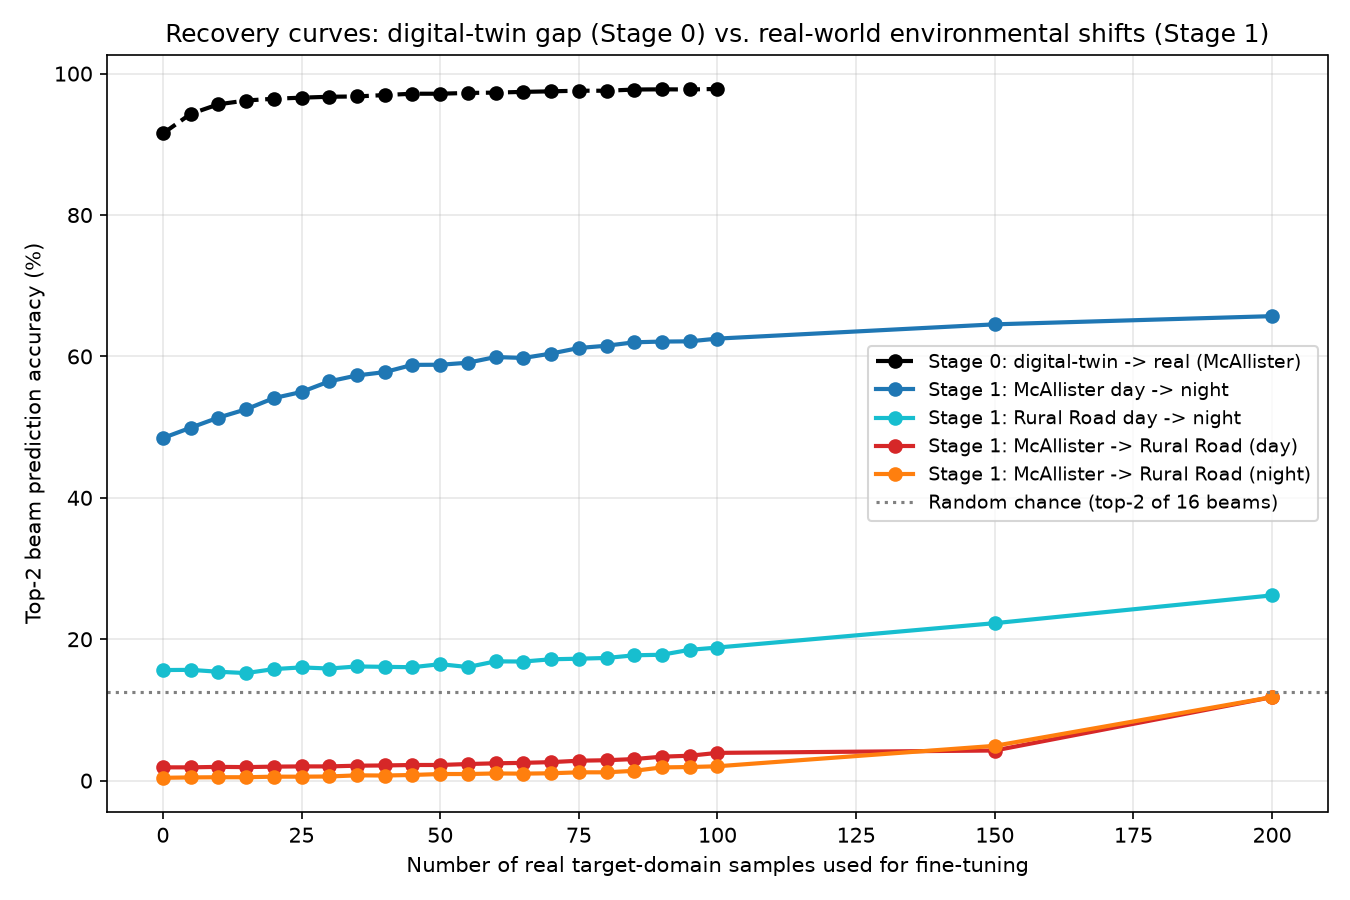
\includegraphics[width=0.95\linewidth]{phase3_recovery_comparison}
    \caption{Top-2 beam prediction accuracy as a function of the number of real fine-tuning samples, for the Stage~0 digital-twin-to-real reproduction and all four Stage~1 real-to-real comparisons, with the 12.5\% random-chance reference line for a 16-class problem.}
    \label{fig:recoverycomparison}
\end{figure}

\autoref{tab:stage1variance} reports the per-seed spread (mean, standard deviation, minimum, and maximum across the 10 seeds) at 100, 150, and 200 real target samples, since the mean values in \autoref{tab:stage1results} alone do not convey how consistently each comparison behaves across independent random data splits.

\begin{table}[H]
    \centering
    \begin{tabular}{c l c c c c}
        \toprule
        Real samples & Comparison & Mean & Std.\ dev. & Min & Max \\
        \midrule
        \multirow{4}{*}{100}
        & McAllister day$\to$night & 62.52\% & 1.62 & 60.34\% & 65.04\% \\
        & Rural Road day$\to$night & 18.82\% & 2.90 & 13.37\% & 25.13\% \\
        & Site shift (day) & 3.93\% & 2.14 & 0.34\% & 6.71\% \\
        & Site shift (night) & 2.03\% & 1.99 & 0.53\% & 6.42\% \\
        \midrule
        \multirow{4}{*}{150}
        & McAllister day$\to$night & 64.54\% & 2.01 & 61.51\% & 68.07\% \\
        & Rural Road day$\to$night & 22.27\% & 3.34 & 16.58\% & 28.61\% \\
        & Site shift (day) & 4.26\% & 1.76 & 0.67\% & 6.38\% \\
        & Site shift (night) & 4.92\% & 3.44 & 0.80\% & 11.23\% \\
        \midrule
        \multirow{4}{*}{200}
        & McAllister day$\to$night & 65.70\% & 1.93 & 62.86\% & 68.74\% \\
        & Rural Road day$\to$night & 26.20\% & 4.18 & 19.52\% & 34.76\% \\
        & Site shift (day) & 11.81\% & 4.13 & 3.69\% & 16.78\% \\
        & Site shift (night) & 11.82\% & 4.39 & 4.28\% & 21.66\% \\
        \bottomrule
    \end{tabular}
    \caption{Per-seed spread of top-2 accuracy (10 seeds) at 100, 150, and 200 real target samples.}
    \label{tab:stage1variance}
\end{table}

\subsection{Data-versus-Optimization Ablation}

\autoref{tab:epochablation} reports the outcome of the epoch-budget ablation described in \autoref{sec:interpretingresults}: for each comparison, the model is fine-tuned on a fixed 100 real target samples, once for the standard 40 epochs and once for a doubled budget of 80 epochs, averaged over 5 random seeds.

\begin{table}[H]
    \centering
    \begin{tabular}{l c c}
        \toprule
        Comparison & 40 epochs & 80 epochs \\
        \midrule
        McAllister day$\to$night & 61.61\% & 61.65\% \\
        Rural Road day$\to$night & 17.17\% & 17.27\% \\
        Site shift (day) & 2.21\% & 2.21\% \\
        Site shift (night) & 1.39\% & 1.44\% \\
        \bottomrule
    \end{tabular}
    \caption{Top-2 accuracy at a fixed 100 real target samples, comparing a 40-epoch and an 80-epoch fine-tuning budget.}
    \label{tab:epochablation}
\end{table}

\subsection{Stage 2: Architecture Comparison}
\label{sec:stage2results}

\autoref{tab:stage2zeroshot} reports the zero-shot (zero real target samples) top-2 accuracy of all four Stage~2 models across the four comparisons, and \autoref{tab:stage2final} reports the same models' top-2 accuracy after two hundred real target samples, the largest sample count swept, under the rehearsal protocol described in \autoref{sec:stage2protocol}. \autoref{fig:stage2recovery} plots the full recovery curve -- accuracy against every swept real-sample count -- for all four models across all four comparisons, and \autoref{fig:stage2bars} presents the two-hundred-sample results of \autoref{tab:stage2final} as a sorted bar chart per comparison for direct visual ranking.

\begin{table}[H]
    \centering
    \begin{tabular}{l c c c c}
        \toprule
        Model & McAllister day$\to$night & Rural Road day$\to$night & Site shift (day) & Site shift (night) \\
        \midrule
        Multi-layer perceptron & 48.45\% & 15.64\% & 1.88\% & 0.40\% \\
        $k$-nearest neighbors & 41.85\% & 14.73\% & 9.26\% & 0.72\% \\
        Random forest & 49.82\% & 13.61\% & 2.35\% & 2.30\% \\
        Fourier + $k$-nearest neighbors & 41.14\% & 12.51\% & 10.60\% & 8.21\% \\
        \bottomrule
    \end{tabular}
    \caption{Zero-shot (zero real target samples) top-2 accuracy for all four Stage~2 models, across all four comparisons. The non-parametric models' zero-shot fit -- on the source scenario alone -- is procedurally identical under both the rehearsal protocol and the discarded target-only protocol described in \autoref{sec:stage2protocol}; small differences from earlier reported values reflect re-running this fit alongside the corrected sweep rather than any change in what is being measured.}
    \label{tab:stage2zeroshot}
\end{table}

\begin{table}[H]
    \centering
    \begin{tabular}{l c c c c}
        \toprule
        Model & McAllister day$\to$night & Rural Road day$\to$night & Site shift (day) & Site shift (night) \\
        \midrule
        Multi-layer perceptron & 65.70\% & 26.20\% & 11.81\% & 11.82\% \\
        $k$-nearest neighbors & 63.98\% & 28.80\% & 48.79\% & 42.46\% \\
        Random forest & \textbf{71.06\%} & \textbf{29.17\%} & \textbf{71.11\%} & \textbf{67.70\%} \\
        Fourier + $k$-nearest neighbors & 62.22\% & 26.66\% & 46.21\% & 38.77\% \\
        \bottomrule
    \end{tabular}
    \caption{Top-2 accuracy at two hundred real target samples for all four Stage~2 models, across all four comparisons, under the rehearsal protocol described in \autoref{sec:stage2protocol}. The best-performing model per comparison is bolded.}
    \label{tab:stage2final}
\end{table}

\begin{figure}[H]
    \centering
    
\includegraphics[width=0.95\linewidth]{model_comparison_recovery_curves}
    \caption{Top-2 beam prediction accuracy as a function of the number of real target-domain samples, for all four Stage~2 models across all four comparisons, with the 12.5\% random-chance reference line for a 16-class problem.}
    \label{fig:stage2recovery}
\end{figure}

\begin{figure}[H]
    \centering
    
\includegraphics[width=0.95\linewidth]{model_comparison_final_accuracy}
    \caption{Top-2 beam prediction accuracy at two hundred real target samples for all four Stage~2 models, sorted by accuracy within each comparison, with the 12.5\% random-chance reference line.}
    \label{fig:stage2bars}
\end{figure}

Two patterns are immediately visible from \autoref{tab:stage2zeroshot} and \autoref{tab:stage2final} and are discussed at length in \autoref{sec:interpretingresults}. First, at zero real target samples, no model is uniformly best: the reference multi-layer perceptron and random forest are the strongest models on the two time-of-day comparisons, while $k$-nearest neighbors and its Fourier-augmented variant are the strongest on the two site-shift comparisons, though all four models remain within roughly the same order of magnitude of each other and of the 12.5\% random-chance level at this point. Second, once any real target-domain samples are available, this picture changes sharply and consistently: random forest outperforms the reference multi-layer perceptron at every sample count greater than zero, across all four comparisons, and $k$-nearest neighbors and its Fourier-augmented variant do the same on both site-shift comparisons specifically; the size of this advantage is largest on the two site-shift comparisons, where the reference multi-layer perceptron plateaus near 11.8\% while random forest reaches 67.7--71.1\% using the same two hundred real samples. Unlike the four comparisons' original, uncorrected numbers, no two comparisons in \autoref{tab:stage2final} that happen to share a target scenario (Rural Road day$\to$night and Site shift (night) both target Scenario~4) are identical: each model's two values for these comparisons now differ by several percentage points, confirming that the rehearsal protocol restores the source scenario's influence at every sweep point rather than discarding it once real target data exists.

\subsection{Stage 3: Extended Site and Lane-Width Comparisons}
\label{sec:stage3results}

\autoref{tab:stage3results} reports zero-shot and two-hundred-sample top-2 accuracy for all eight Stage~3 comparisons, averaged over ten random seeds, using the identical reference multi-layer perceptron and protocol as Stage~1.

\begin{table}[H]
    \centering
    \begin{tabular}{c l c c c c}
        \toprule
        Label & Comparison & Lane width & 0 samples & 100 samples & 200 samples \\
        \midrule
        R1 & Scenario~2 $\to$ 1 & Same & 52.09\% & 63.23\% & 69.13\% \\
        R2 & Scenario~4 $\to$ 2 & Different & 6.02\% & 7.43\% & 14.15\% \\
        R3 & Scenario~1 $\to$ 32 & Same & 19.95\% & 24.19\% & 35.27\% \\
        R4 & Scenario~32 $\to$ 1 & Same & 11.35\% & 16.40\% & 21.53\% \\
        R5 & Scenario~1 $\to$ 33 & Same & 12.26\% & 11.00\% & 21.27\% \\
        R6 & Scenario~33 $\to$ 1 & Same & 10.37\% & 14.16\% & 20.72\% \\
        R7 & Scenario~1 $\to$ 7 & Different & 2.63\% & 2.63\% & 5.96\% \\
        R8 & Scenario~7 $\to$ 1 & Different & 3.50\% & 5.11\% & 16.99\% \\
        \bottomrule
    \end{tabular}
    \caption{Top-2 accuracy for all eight Stage~3 comparisons, averaged over 10 random seeds, using the reference multi-layer perceptron and the identical protocol used throughout Stage~1.}
    \label{tab:stage3results}
\end{table}

Two patterns follow directly from \autoref{tab:stage3results}. First, comparison~R1, the reverse of the original McAllister time-of-day comparison, recovers to 69.13\% at two hundred samples, close to and consistent with the corresponding forward-direction Stage~1 result (65.70\%, \autoref{tab:stage1results}); comparison~R2, the reverse of the original nighttime site-shift comparison, reaches only 14.15\%, closely consistent with the corresponding forward-direction result (11.82\%). Both reverse-direction checks therefore confirm that the original Stage~1 findings are not an artifact of the specific source-to-target direction originally tested, in either the mild time-of-day case or the severe site-shift case. Second, averaging the four same-lane-width comparisons (R3--R6: 35.27, 21.53, 21.27, and 20.72\% at two hundred samples) against the four different-lane-width comparisons (R7--R8, plus the original Stage~1 site-shift comparisons 1$\to$3 and 2$\to$4 reported in \autoref{tab:stage1results}, which also change lane width) shows same-lane-width comparisons recovering to a mean of 24.70\% at two hundred samples, against a mean of 12.30\% for different-lane-width comparisons -- roughly double. This pattern is directional-symmetry-robust: it holds in both the forward direction (R3, R5 against R7) and the reverse direction (R4, R6 against R8), which rules out the possibility that the gap is an artifact of one direction happening to be easier than the other for unrelated reasons. Lane width, independent of site identity, therefore behaves as a real, measurable contributor to site-shift severity, though \autoref{sec:stage4findings} and \autoref{sec:interpretingresultsstage3} show this picture requires substantial further qualification once the underlying data itself is examined.

Also of note is the shape of the different-lane-width recovery curves, not only their endpoint: comparison~R7 (Scenario~1 $\to$ 7) records accuracy that is effectively flat at 2.63\% top-2 accuracy from zero samples through one hundred samples, with the full 23-point sweep visually indistinguishable from a flat line until a modest rise to 5.96\% appears only at the two largest sweep points (150 and 200 samples); comparison~R8 shows a similarly delayed rise, from 3.5\% at zero samples to only 5.1\% at one hundred, before a comparable late increase to 16.99\% at two hundred. By contrast, the same-lane-width comparison~R3 begins moving within the first five real samples (from 19.95\% at zero samples to 22.55\% at five). This suggests that a lane-width mismatch does not only depress the ceiling that fine-tuning can reach within the sample range tested, but delays the point at which fine-tuning begins to have any measurable effect at all.

\subsection{Stage 4: Diagnosing and Partially Resolving the College Ave Instability}
\label{sec:stage4findings}

\subsubsection{Per-Seed Trajectories Reveal Genuine Training Instability, Not Sampling Noise}

Comparisons~R3 and~R5 (Scenario~1 as source, Scenarios~32 and~33 as target) exhibit a standard deviation across seeds of 7.1 and 12.1 percentage points respectively at two hundred samples, several times larger than any Stage~1 comparison at the same sample count (\autoref{tab:stage1variance}: 1.93 to 4.39). Disaggregating comparison~R3 into its ten individual seed trajectories, rather than reporting only this aggregate spread, shows the following. Two seeds are frozen at a constant accuracy, to within one decimal place, across the \emph{entire} sweep from zero to two hundred samples (30.0\% and 30.3--30.4\%, respectively): two hundred real fine-tuning samples produce no measurable change in test-set behavior for these particular random initializations and data draws. A third seed's own trajectory is non-monotonic -- rising from 3.4\% at zero samples to 31.2\% at fifteen samples, falling back to 3.7\% at fifty and seventy samples, then climbing again to 21.0\% by two hundred samples -- indicating that a specific small-sample draw actively degraded this seed's fine-tuned model relative to an earlier, larger-looking result, rather than simply providing insufficient additional information. A fourth seed remains flat near 30\% for the first twenty-one sweep points before dropping to 4.8\% at exactly 150 samples and recovering to 37.2\% at 200. Comparison~R5 shows the same qualitative pattern in different seeds: one seed remains near 2--4\% for the entire sweep; two others sit flat in the 12--18\% range for most of the sweep before jumping sharply, at the very last sweep point, to 43.9\% and 46.2\% respectively -- meaning the reported 21.27\% mean at two hundred samples for R5 is disproportionately driven by two of ten seeds, while the remaining eight sit considerably lower. This is the same failure mode, in a more extreme form, that motivated the five-to-ten seed correction described in \autoref{sec:interpretingresults} for the original site-shift comparisons, and indicates the R3/R5 means in \autoref{tab:stage3results} should be read as considerably less representative of a ``typical'' outcome than the corresponding standard deviations alone would suggest.

\subsubsection{GPS Position-Quality Metadata Differs Sharply from Scenario 1}

Examining the raw DeepSense~6G development CSV metadata for Scenarios~32 and~33 confirms a concrete, quantifiable data-quality difference absent from Scenario~1. \autoref{tab:gpsquality} reports the fraction of samples in each scenario whose recorded position was either interpolated (the receiver failed to obtain a fix at that timestamp) or reported with an invalid fix type without being flagged as interpolated.

\begin{table}[H]
    \centering
    \begin{tabular}{c c c c}
        \toprule
        Scenario & Fix type & Interpolated positions & Degraded-position fraction \\
        \midrule
        1 (McAllister) & 100\% valid 3D fix & 0 of 2411 (no such field) & 0.0\% \\
        32 (College Ave.) & 2880 valid / 55 invalid (fix type 0) & 300 of 3235 & 11.0\% \\
        33 (College Ave.) & 3616 valid / 63 invalid (fix type 0) & 302 of 3981 & 9.2\% \\
        \bottomrule
    \end{tabular}
    \caption{GPS position-quality metadata for Scenario~1 versus Scenarios~32 and~33, drawn directly from each scenario's raw DeepSense~6G development CSV file.}
    \label{tab:gpsquality}
\end{table}

Scenario~1's CSV contains no interpolated-position field at all, and every one of its samples carries a valid three-dimensional GPS fix. Scenarios~32 and~33, by contrast, have approximately 9--11\% of their samples drawn from a position that was either interpolated from surrounding fixes or recorded despite an explicitly invalid fix type, and the preprocessing pipeline described in \autoref{sec:data} does not filter, weight, or otherwise treat these samples any differently from a fully measured one. Because the fine-tuning sweep at small sample counts (as few as five samples) draws directly from this pool without regard to position quality, a small draw that happens to include one or more of these degraded-position samples carries a disproportionately large, and disproportionately misleading, share of the gradient signal used to fine-tune the model at that sweep point -- a plausible mechanistic explanation for the non-monotonic, seed-specific collapses documented in the previous subsection.

Beam-label class balance differs between the sites in a related and compounding way. Computing the fraction of samples whose optimal beam is the single most common beam observed at that scenario gives 12.0\% for Scenario~1, but 27.1\% and 29.0\% for Scenarios~32 and~33 respectively; the three most common beams jointly account for 27.8\% of Scenario~1's samples but 48.8\% and 54.2\% of Scenarios~32 and~33's samples. A small random draw from a more class-imbalanced pool is correspondingly more likely to omit several of the rarer beam classes entirely, or to include several examples of only the majority class, either of which would leave a fine-tuning run with no useful gradient signal for the omitted classes -- consistent with the frozen, unresponsive seed trajectories documented above.

\subsubsection{The Road at College Avenue Physically Curves; the Road Used for Comparison R7/R8 Does Not}

Applying the five-meter-bin cross-road standard deviation diagnostic described in \autoref{sec:stage4geometry} to Scenarios~32 and~33 reveals a sharp, unambiguous geometric signature. \autoref{tab:bendevidence} reports representative bins from this analysis for Scenario~32; Scenario~33 shows the same pattern at the same along-road coordinate.

\begin{table}[H]
    \centering
    \begin{tabular}{c c c c}
        \toprule
        Along-road coordinate bin (m) & Samples & Cross-road std.\ dev.\ (m) & Cross-road range (m) \\
        \midrule
        $[20, 25)$ & 270 & 1.94 & [14.2, 19.0] \\
        $[30, 35)$ & 381 & 1.77 & [14.0, 19.1] \\
        $[35, 40)$ & 675 & 1.51 & [13.8, 19.0] \\
        $[40, 45)$ & 231 & 2.38 & [12.6, 19.0] \\
        $[45, 50)$ & 503 & 4.14 & [3.1, 18.1] \\
        $[50, 55)$ & 127 & 3.05 & [2.3, 14.0] \\
        \bottomrule
    \end{tabular}
    \caption{Cross-road position standard deviation per five-meter along-road bin, Scenario~32. The cross-road spread nearly triples beginning at the $[45,50)$~m bin, the geometric signature of the road curving away from its dominant heading.}
    \label{tab:bendevidence}
\end{table}

The cross-road standard deviation stays tight and stable, between 1.5 and 2.4~m, for every bin below approximately 40~m along the road, then increases sharply, to 4.14~m and 3.05~m in the final two bins, exactly where the vehicle's recorded cross-road position spans nearly the full 3--19~m range rather than the roughly 14--19~m range observed throughout the rest of the segment. \autoref{fig:scenario32full} and \autoref{fig:scenario33full} show this directly: both scenarios' captured road segments visibly curve away from their dominant heading beyond approximately 40~m from the base station's along-road reference point, a geometric property entirely absent from every other scenario in this thesis, including Scenario~7 (\autoref{fig:scenario7scatter}), whose road is a straight, diagonally-oriented segment relative to its base station rather than a curved one, and Scenario~1 (\autoref{fig:scenario1scatter}), reproduced here for direct visual comparison.

\begin{figure}[H]
    \centering
    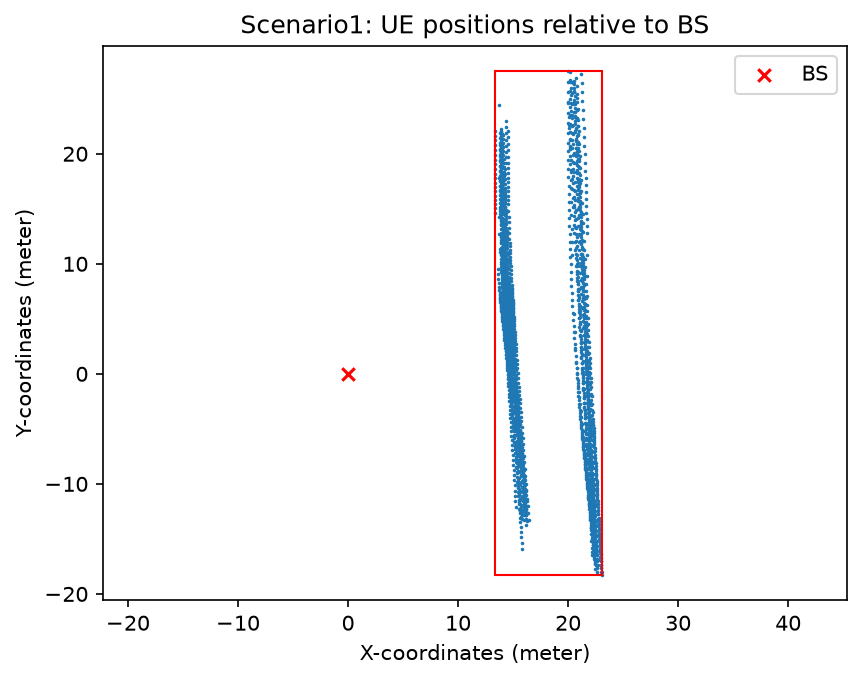
\includegraphics[width=0.72\linewidth]{scenario1_ue_scatter}
    \caption{Scenario~1 (McAllister Ave.) UE positions relative to the base station: a straight, tightly bounded two-lane segment, included here for direct visual comparison with \autoref{fig:scenario32full} and \autoref{fig:scenario33full}.}
    \label{fig:scenario1scatter}
\end{figure}

\begin{figure}[H]
    \centering
    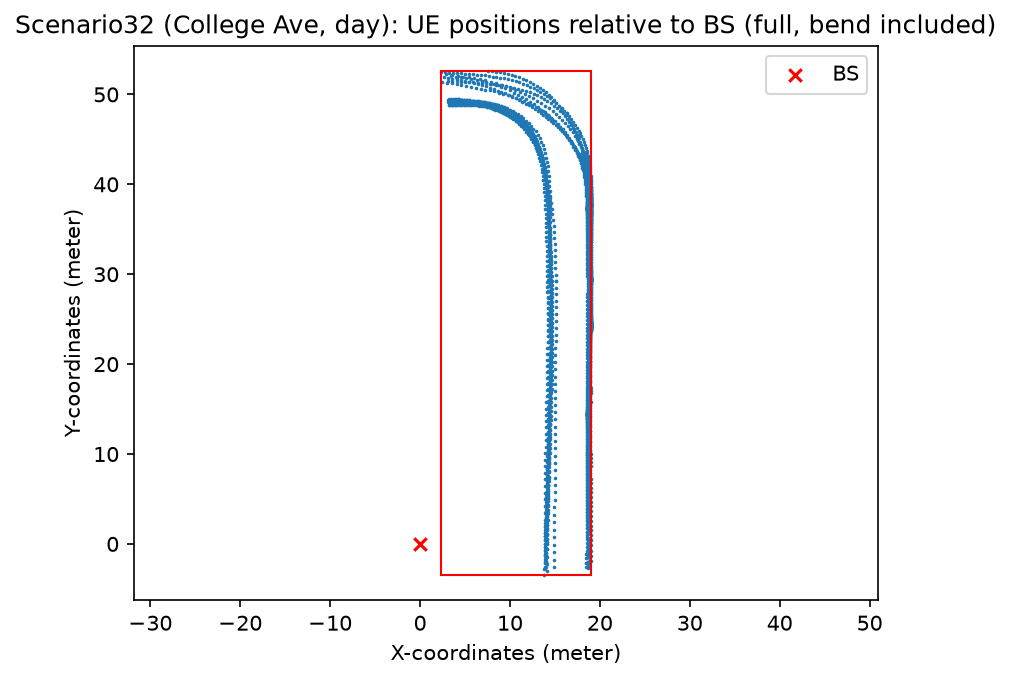
\includegraphics[width=0.72\linewidth]{scenario32_full_ue_scatter}
    \caption{Scenario~32 (College Ave., day) UE positions relative to the base station, full data. The road visibly curves beyond approximately 40~m along the road, unlike Scenario~1.}
    \label{fig:scenario32full}
\end{figure}

\begin{figure}[H]
    \centering
    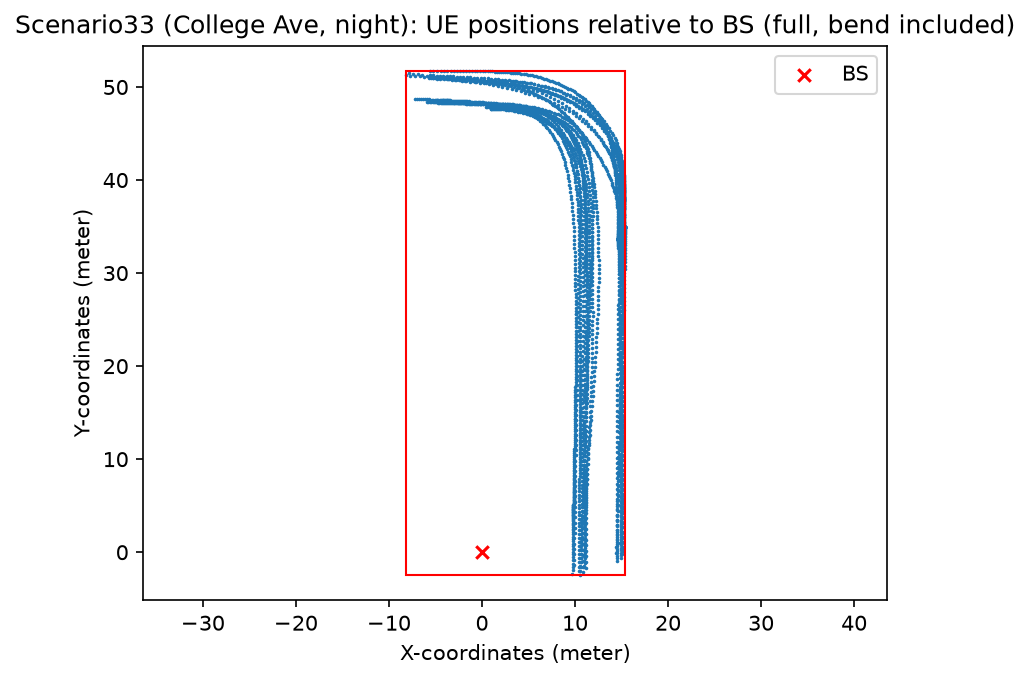
\includegraphics[width=0.72\linewidth]{scenario33_full_ue_scatter}
    \caption{Scenario~33 (College Ave., night) UE positions relative to the base station, full data, showing the same curve at the same along-road coordinate as Scenario~32.}
    \label{fig:scenario33full}
\end{figure}

\begin{figure}[H]
    \centering
    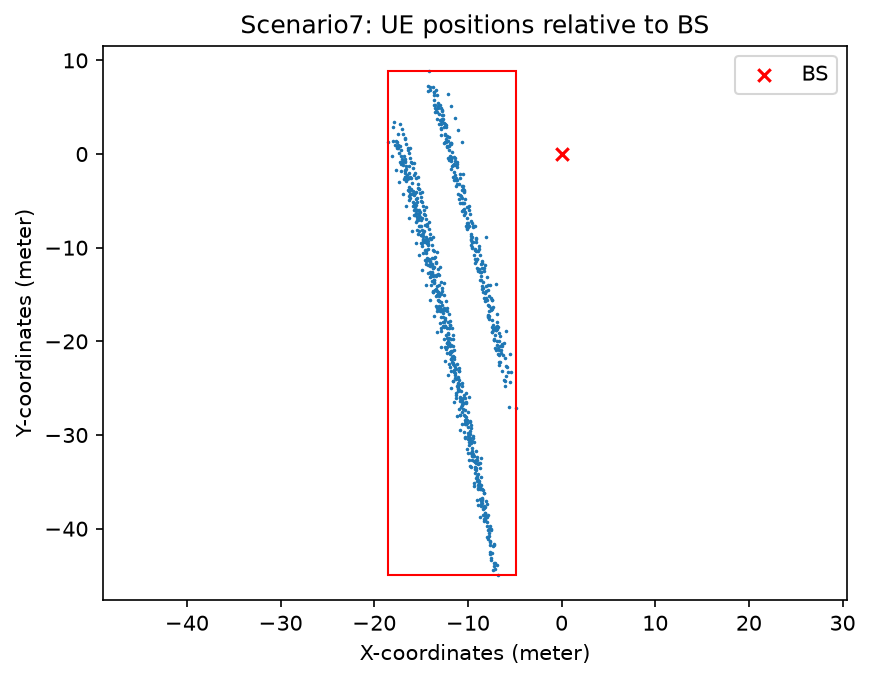
\includegraphics[width=0.72\linewidth]{scenario7_ue_scatter}
    \caption{Scenario~7 UE positions relative to the base station: a straight road segment oriented diagonally relative to the base station's coordinate frame, included to confirm that Scenario~7's severe recovery result (comparisons~R7/R8) is not confounded by the same road-curvature property found in Scenarios~32 and~33.}
    \label{fig:scenario7scatter}
\end{figure}

This is a materially important finding for interpreting comparisons~R3 through~R6: the ``same lane width'' comparisons built from Scenario~1 and Scenarios~32/33 are not, in fact, comparisons between two otherwise-equivalent straight roads. They additionally differ in road geometry, a variable the original Stage~1 design and the Stage~3 lane-width extension did not anticipate or control for. Because comparisons~R7 and~R8 (the different-lane-width comparisons using Scenario~7) do \emph{not} share this confound, the width-versus-orientation conclusion drawn from \autoref{tab:stage3results} above rests on cleaner ground for R7/R8 than it does for R3--R6.

\subsubsection{Removing the Curve Helps, but Mainly When the Curved Site Is the Deployment Target}

Filtering Scenarios~32 and~33 to only the samples below the 40~m along-road cutoff identified above retains 2374 of 3235 samples (73.4\%) for Scenario~32 and 2574 of 3981 samples (64.7\%) for Scenario~33; \autoref{fig:scenario32straight} and \autoref{fig:scenario33straight} show the resulting straight-only position scatter for each, both now visually comparable in shape to Scenario~1. \autoref{tab:straightvsfull} reports the resulting Stage~4 comparisons (\autoref{tab:stage4straightcomparisons}) alongside their full-data Stage~3 counterparts.

\begin{figure}[H]
    \centering
    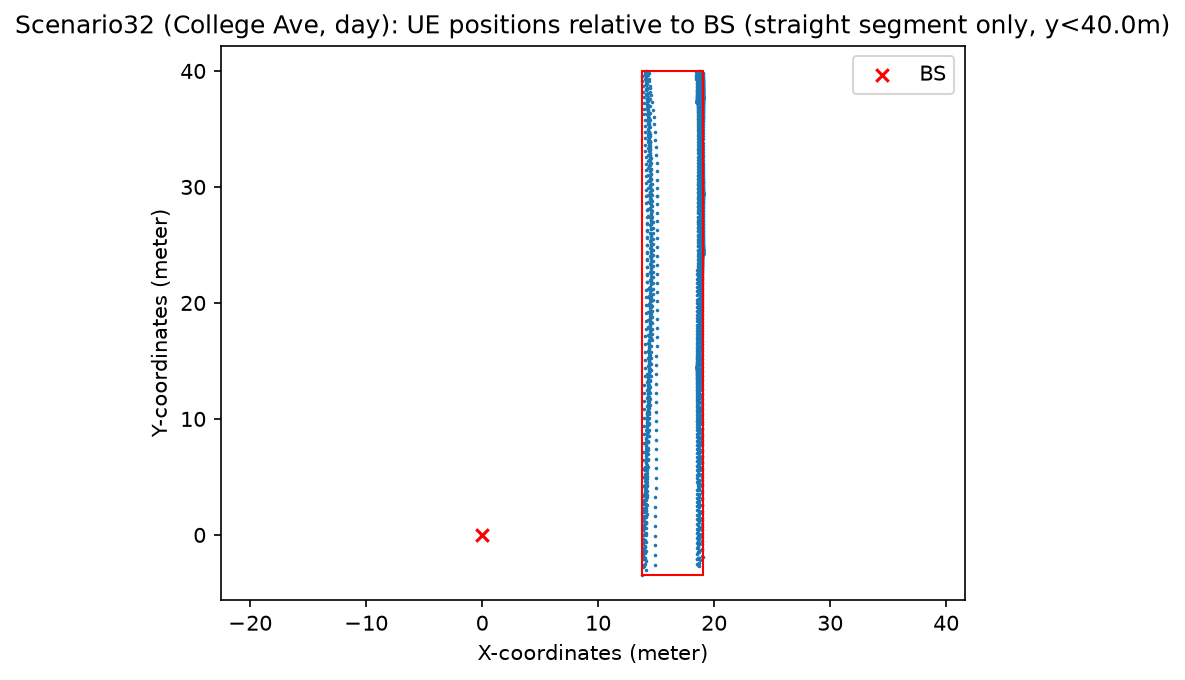
\includegraphics[width=0.72\linewidth]{scenario32straight_ue_scatter}
    \caption{Scenario~32, restricted to the straight segment only (along-road coordinate below 40~m). Compare with the full-data version in \autoref{fig:scenario32full}.}
    \label{fig:scenario32straight}
\end{figure}

\begin{figure}[H]
    \centering
    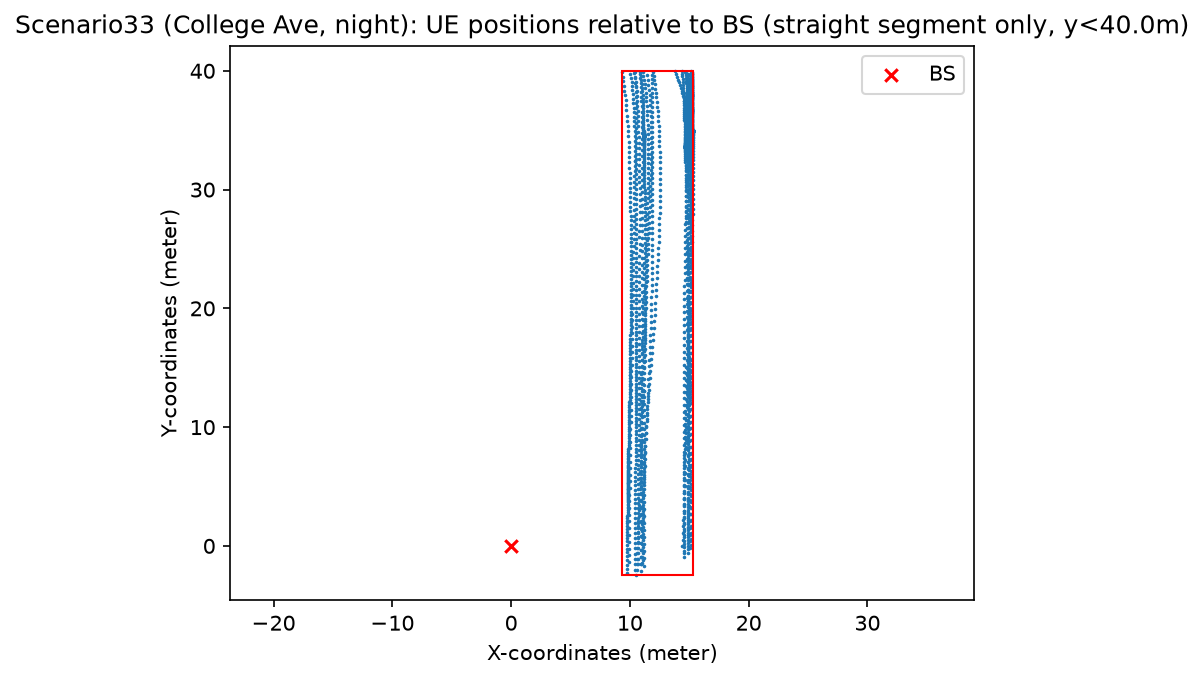
\includegraphics[width=0.72\linewidth]{scenario33straight_ue_scatter}
    \caption{Scenario~33, restricted to the straight segment only (along-road coordinate below 40~m). Compare with the full-data version in \autoref{fig:scenario33full}.}
    \label{fig:scenario33straight}
\end{figure}

\begin{table}[H]
    \centering
    \begin{tabular}{c l c c c c c}
        \toprule
        Label & Comparison & 0 samples & 100 samples & 200 samples & Std.\ dev.\ at 200 (full) & Std.\ dev.\ at 200 (straight) \\
        \midrule
        R3 / S3 & Scenario~1 $\to$ 32 & 19.95 / 32.13 & 24.19 / 35.91 & 35.27 / 40.90 & 7.1 & 5.1 \\
        R4 / S4 & Scenario~32 $\to$ 1 & 11.35 / 10.32 & 16.40 / 14.10 & 21.53 / 17.79 & 3.9 & 2.0 \\
        R5 / S5 & Scenario~1 $\to$ 33 & 12.26 / 7.72 & 11.00 / 11.65 & 21.27 / 22.72 & 12.1 & 15.1 \\
        R6 / S6 & Scenario~33 $\to$ 1 & 10.37 / 11.05 & 14.16 / 18.53 & 20.72 / 25.51 & 4.7 & 3.7 \\
        \bottomrule
    \end{tabular}
    \caption{Full-data (R3--R6) versus straight-segment-only (S3--S6) top-2 accuracy, reported as full~/~straight pairs at each sample count.}
    \label{tab:straightvsfull}
\end{table}

The effect of removing the curve is not uniform across the four comparisons, and the pattern it follows is itself informative. Comparison~R3/S3 (McAllister$\to$College~Ave.\ day) improves on both accuracy and stability simultaneously: mean accuracy rises at every sample count (19.95\% to 32.13\% at zero samples, 35.27\% to 40.90\% at two hundred), and the standard deviation at intermediate sample counts (30 to 100 samples) falls to as low as 2.1--2.5 percentage points, from 9--10 for the full-data version. Comparison~R6/S6 (College~Ave.\ night$\to$McAllister) improves similarly across the entire sweep (20.72\% to 25.51\% at two hundred samples) with comparably low standard deviation in both versions. Comparison~R5/S5 (McAllister$\to$College~Ave.\ night), however, shows a more qualified improvement: standard deviation at 70--90 samples falls dramatically, from 4.8--5.6 to 0.9--1.1 percentage points, but standard deviation at two hundred samples \emph{rises}, from 12.1 to 15.1. Disaggregating S5's two-hundred-sample seeds individually shows two seeds jumping to 64.9\% and 32.0\% while the remaining eight sit between 13\% and 24\% -- the same late-jump pattern documented for R5 above, but occurring in a different pair of seeds. Since the GPS-quality analysis in \autoref{tab:gpsquality} found that the interpolated and invalid-fix samples for both Scenarios~32 and~33 are concentrated mainly in the straight portion of the road, not the curved portion (258 of 355 degraded samples for Scenario~32, 250 of 365 for Scenario~33), this residual instability in S5 is consistent with the still-unfiltered GPS-quality issue rather than with the curve, which S5's data no longer contains.

Comparison~R4/S4 (College~Ave.\ day$\to$McAllister) is the sole case in which removing the curve does not help: mean accuracy is slightly \emph{lower} for S4 than for R4 at every sample count (10.32\% versus 11.35\% at zero samples, 17.79\% versus 21.53\% at two hundred), though the standard deviation at two hundred samples is somewhat lower for S4 (2.0 versus 3.9). This asymmetry is consistent with a specific, mechanistic account of what the curve actually damages: in R4/S4, College Avenue plays only the \emph{source} role, supplying the pretraining pool, while McAllister -- a site whose road is straight in every scenario used throughout this thesis -- plays the \emph{target} role that is actually evaluated and fine-tuned on. Removing 861 samples from the source pretraining pool, without correspondingly removing any evaluation-side ambiguity (since the evaluation target, McAllister, was never curved to begin with), simply reduces the amount of information available to the pretraining step, with no confound left on the evaluation side to fix. R3/S3, R5/S5, and R6/S6, by contrast, all place a College Avenue scenario in the target role at some point in their protocol (R3/S3 and R5/S5 as the fine-tuning and evaluation target directly; R6/S6 as the scenario supplying the source-domain training pool that a model is trained from scratch on, which still determines what decision boundary the model learns before ever seeing McAllister). This asymmetry -- an improvement specifically when the curved site is being generalized \emph{to}, and no corresponding improvement when the curved site is only feeding the source training pool -- is stronger evidence for a genuine causal mechanism than a uniform improvement across all four comparisons would have been, since a uniform improvement would be equally consistent with the simpler, less interesting explanation that removing 26--35\% of a scenario's noisiest data improves results for any reason at all, regardless of source or target role.

\subsubsection{Base Station Orientation at College Avenue Differs From McAllister by Roughly Forty Degrees}

Applying the center-beam orientation estimation procedure (\autoref{sec:data}, \autoref{sec:stage4orientation}) to Scenarios~32 and~33 for the first time in this thesis produces the estimates in \autoref{tab:collegeorientation}, alongside the previously reported Scenario~1 and~2 estimates for direct comparison.

\begin{table}[H]
    \centering
    \begin{tabular}{c l c c}
        \toprule
        Scenario & Site / Time & Orientation & Center-beam samples \\
        \midrule
        1 & McAllister Ave., Day & $9.70^\circ$ & 42 \\
        2 & McAllister Ave., Night & $5.04^\circ$ & 83 \\
        32 (full data) & College Ave., Day & $49.10^\circ$ & 67 \\
        32 (straight only) & College Ave., Day & $44.70^\circ$ & 58 \\
        33 & College Ave., Night & $55.15^\circ$ & 89 \\
        \bottomrule
    \end{tabular}
    \caption{Base station orientation estimates for Scenarios~1, 2, 32, and~33, using the center-beam least-squares procedure described in \autoref{sec:data}. Scenario~33's estimate is identical for the full and straight-only data, indicating all of its center-beam samples happen to lie on the straight segment.}
    \label{tab:collegeorientation}
\end{table}

McAllister Avenue's base station is oriented at approximately $5$--$10^\circ$; College Avenue's is oriented at approximately $45$--$55^\circ$, a difference of roughly $35$ to $45$ degrees -- several times larger than the $6$ to $13$ degree spread previously measured among Scenarios~1 through~4 in \autoref{sec:interpretingresults}, and, for a sixteen-beam codebook in which each beam spans approximately $22.5^\circ$ of angle, equivalent to roughly two entire beam-widths of mismatch. This provides a direct, quantitative answer to why comparisons~S3 and~S4 still recover to only 40.90\% and 17.79\% respectively at two hundred samples even after the curved portion of the road, and the instability it produced, has been removed entirely: removing the curve addresses the local, small-sample training instability documented earlier in this section, but does not, and cannot, address this much larger, purely orientation-driven component of the site-shift difficulty, since it reflects a difference in the physical mounting of the two sites' hardware rather than any property of the road geometry or data quality that preprocessing could correct for. This also situates College Avenue's orientation gap as the single largest documented in this thesis, exceeding even the gap between McAllister and Rural Road that originally motivated the orientation-mismatch explanation in \autoref{sec:interpretingresults}, and it is discussed further, alongside the R7/R8 width-mismatch result, in \autoref{sec:interpretingresultsstage3}.

\subsection{Stage 5: The Non-Parametric Rehearsal Advantage Under Lane-Width Mismatch}
\label{sec:stage5results}

\autoref{tab:stage5results} reports zero-shot and two-hundred-sample top-2 accuracy for all six Stage~5 comparisons and all three rehearsal-trained non-parametric models.

\begin{table}[H]
    \centering
    \begin{tabular}{l c c c c c c}
        \toprule
        & \multicolumn{2}{c}{$k$-NN} & \multicolumn{2}{c}{Random forest} & \multicolumn{2}{c}{Fourier + $k$-NN} \\
        Comparison & 0 & 200 & 0 & 200 & 0 & 200 \\
        \midrule
        McAllister day $\to$ Scenario~7            & 10.53\% & 52.63\% & 2.28\% & 76.08\% & 11.23\% & 52.28\% \\
        McAllister day $\to$ College Ave.\ day     & 0.25\%  & 73.77\% & 0.25\% & 83.33\% & 3.98\%  & 73.85\% \\
        McAllister day $\to$ College Ave.\ night   & 0.54\%  & 77.94\% & 0.54\% & 88.21\% & 2.72\%  & 77.11\% \\
        McAllister night $\to$ Scenario~7          & 6.78\%  & 52.57\% & 5.26\% & 75.38\% & 11.40\% & 52.16\% \\
        McAllister night $\to$ College Ave.\ day   & 0.15\%  & 75.58\% & 4.51\% & 82.15\% & 6.36\%  & 75.75\% \\
        McAllister night $\to$ College Ave.\ night & 0.56\%  & 75.96\% & 0.83\% & 84.80\% & 2.68\%  & 75.22\% \\
        \bottomrule
    \end{tabular}
    \caption{Top-2 accuracy at zero and two hundred real target samples for all six Stage~5 comparisons, averaged over 10 random seeds, under the rehearsal protocol of \autoref{sec:stage2protocol}. College Avenue targets use the curvature-free straight-segment data from Stage~4.}
    \label{tab:stage5results}
\end{table}

Two patterns follow directly from \autoref{tab:stage5results}, and both extend the Stage~2 finding rather than qualifying it. First, random forest is again the strongest model on every one of the six comparisons, reaching 75.38--88.21\% top-2 accuracy at two hundred samples -- comparable to, and on the College Avenue comparisons noticeably higher than, its 67.70--71.11\% on the original Stage~1 site-shift comparisons in \autoref{tab:stage2final}. $k$-nearest neighbors and its Fourier-augmented variant again trail random forest but still reach 52--78\% across every comparison, far above the corresponding reference-multi-layer-perceptron results reported for the same site pairs in \autoref{tab:stage3results}: comparisons~R7 and~R8 (Scenario~1/Scenario~7, the identical narrow-to-wide site pair used in the first row of \autoref{tab:stage5results}) reach only 5.96\% and 16.99\% at two hundred samples for the reference model, against 52.63\% and 52.57\% for rehearsal-trained $k$-nearest neighbors on the corresponding forward and reverse-role comparisons here. Second, this advantage holds specifically on the exact site pair -- McAllister versus Scenario~7 -- that \autoref{sec:interpretingresultsstage3} identifies as the cleanest available test of lane-width mismatch, since Scenario~7's road is straight and its orientation-versus-McAllister difference has not been separately measured; the non-parametric rehearsal advantage is therefore not confined to the narrower range of site differences present in the original four-scenario Stage~1/Stage~2 design, and persists on a site pair the reference model itself found the single hardest to recover on in \autoref{tab:stage3results}.

\section{Interpreting the Results}
\label{sec:interpretingresults}

\subsection{Stage 0 Validates the Pipeline}

The reproduced zero-shot top-2 accuracy of 91.53\% is within 0.13 percentage points of the originally published 91.4\%, and the recovery trajectory this thesis obtains -- rapid improvement within the first twenty real samples, followed by a much flatter approach toward 100 samples -- reproduces the qualitative shape of the previously published curve. This confirms that the model architecture, training procedure, and evaluation metrics implemented for this thesis behave as expected before being repurposed for the Stage~1 questions this thesis actually investigates, and it rules out the possibility that any Stage~1 finding is an artifact of a faulty reimplementation of the underlying pipeline.

\subsection{Zero-Shot Degradation Differs in Kind, Not Only in Degree, Between Shift Types}

Expressed relative to the 12.5\% random-chance baseline for this 16-class problem, the two shift types produce categorically different zero-shot outcomes. The McAllister time-of-day shift retains 48.45\% zero-shot accuracy, 3.9 times the chance level; the Rural Road time-of-day shift retains 15.64\%, 1.25 times chance. Both site-shift comparisons, in contrast, fall far below chance: 1.88\% (0.15 times chance) for the daytime site shift and 0.40\% (0.03 times chance) for the nighttime site shift. A model performing below random chance is not merely uncertain -- a uniformly random predictor would already achieve 12.5\% -- it is confidently and systematically wrong, consistently favoring beams that are not correct for the new site. This is consistent with the two sites' base stations being mounted at measurably different absolute orientations (estimated at $12.20^\circ$ and $5.53^\circ$ for the two McAllister scenarios and $9.32^\circ$ and $-1.05^\circ$ for the two Rural Road scenarios, using the center-beam estimation procedure described in \autoref{sec:data}), which would cause the same beam index to correspond to a different physical pointing direction at the two sites; a model that has learned a smooth, confident mapping from position to beam index at one site would then apply that mapping to a set of coordinates for which it corresponds to a systematically incorrect answer at the other site, rather than to a merely unfamiliar one. A supplementary check of the per-scenario best-beam label distributions found only partial support for this explanation: the two sites' most frequently optimal beams overlap in only one of their top three choices, but a simple calculation shows that a model defaulting only to McAllister's most common beams would still be expected to score near the chance level at Rural Road, not substantially below it, indicating that the mismatch lies in the structure of the position-to-beam mapping itself rather than only in a difference in which beams are used how often.

\subsection{The Orientation-Mismatch Failure Is Specific to the Fine-Tuning Recipe, Not Intrinsic to the Site-Shift Task}

The Stage~2 results directly resolve the two-way ambiguity raised in \autoref{sec:stage2}: whether the severe, below-chance site-shift degradation described above is an unavoidable property of the site-shift task, or a property specific to the reference multi-layer perceptron's gradient-based fine-tuning recipe. \autoref{tab:stage2final} shows it is predominantly the latter. At two hundred real target samples, random forest reaches 71.11\% top-2 accuracy on the daytime site shift and 67.70\% on the nighttime site shift, against the reference multi-layer perceptron's 11.81\% and 11.82\% on the same two comparisons -- a difference of roughly sixty percentage points using the identical amount of real target data, and using an equally weighted mixture of that same real target data with the full source pool rather than the target data alone. $k$-nearest neighbors and its Fourier-augmented variant show the same qualitative pattern, reaching 48.79\% and 46.21\% respectively on the daytime site shift and 42.46\% and 38.77\% on the nighttime site shift, so this is not an idiosyncrasy of one non-parametric method but a property shared across every non-parametric model tested, even though random forest's specific advantage over the other two is itself substantial.

This pattern is consistent with, and strengthens, the orientation-mismatch mechanism proposed above. A gradient-trained neural network converges, during source-domain training, to a single smooth global function from position to beam index; fine-tuning that same network on a small number of target-domain samples adjusts its weights incrementally from that starting point but does not force it to discard the globally confident, source-specific rule it has already learned, particularly when the number of new gradient steps is small relative to the number of steps spent learning the original rule. A $k$-nearest-neighbors or random-forest model fit at a given real-sample sweep point, by contrast, is refit from scratch on the full source-plus-target rehearsal set described in \autoref{sec:stage2protocol}, so it carries no \emph{persisted} state from any previous fit: it re-weighs the same source evidence the neural model's checkpoint was pretrained on directly against the target evidence at every sweep point, rather than having to incrementally overwrite a set of weights already committed to a source-specific rule. The Stage~2 results are therefore best read not as showing that random forest or $k$-nearest neighbors is unconditionally a better model for this task, or that these models are simply given more information than the neural model -- \autoref{sec:stage2protocol} establishes that, under rehearsal, they are not -- but as showing that \emph{how} source and target evidence are combined matters as much as how much of each is available: committing to a smooth, globally-fit decision function via gradient descent and then incrementally adjusting it is precisely what makes a site shift so costly to recover from, and that cost is avoidable by a model that recombines the same evidence from scratch at every step, not an unavoidable property of the change in site itself.

The Fourier-augmented variant of $k$-nearest neighbors complicates this picture in an informative way rather than contradicting it. At zero real target samples, it achieves the higher accuracy of the two $k$-nearest-neighbors variants on both site-shift comparisons (10.60\% and 8.21\%, against 9.26\% and 0.72\% for plain $k$-nearest neighbors), suggesting the sinusoidal position encoding does provide some useful structure to a model fit only on source-domain data. At every real-sample count greater than zero, however, the Fourier-augmented variant trails plain $k$-nearest neighbors on every comparison in \autoref{tab:stage2final} -- 46.21\% against 48.79\% on the daytime site shift, 38.77\% against 42.46\% on the nighttime site shift. This is consistent with the dimensionality argument raised in \autoref{sec:fourierstage2}: expanding a 4-dimensional input to 28 dimensions provides no benefit if the underlying model already makes no smoothness assumption for the encoding to correct, and instead leaves a fixed real-sample budget -- as few as five real target samples at the smallest sweep point, rehearsed alongside a source pool whose size does not change with the encoding -- to constrain a substantially larger feature space, which is a well-documented risk to generalization independent of this specific task.

\subsection{Real Data, Not Optimization Budget, Drives Recovery}

The clearest evidence for what drives recovery comes from the contrast between \autoref{tab:stage1results} and \autoref{tab:epochablation}. Between 100 and 200 real target samples, accuracy for the two site-shift comparisons rises from 3.93\% to 11.81\% and from 2.03\% to 11.82\% respectively -- increases of roughly 8 and 10 percentage points. Yet doubling the fine-tuning epoch budget at a fixed 100 real samples changes accuracy by less than 0.1 percentage points for every comparison, including the two site-shift comparisons (2.21\% to 2.21\%, and 1.39\% to 1.44\%). Since increasing the real-sample count from 100 to 200 also roughly doubles the number of gradient updates performed within a fixed 40-epoch fine-tuning run (more samples produce more batches per epoch at a fixed batch size of 8), this ablation was necessary to rule out the possibility that the observed recovery was simply an artifact of more optimization steps rather than more informative data. The ablation shows this is not the case: additional real data, not additional training time, is what allows the model to escape a badly-mismatched initialization.

\subsection{Internal Consistency, and a Correction the Data Itself Produced}

The two site-shift comparisons, despite being measured independently -- at different times of day, using different held-out test partitions -- converge to nearly identical accuracy at 200 real samples (11.81\% and 11.82\%), which is strong evidence that the site-shift effect is a genuine, repeatable property of the site change itself rather than an artifact of one particular comparison. The two time-of-day comparisons do not converge to similar absolute accuracy (65.70\% versus 26.20\% at 200 samples), but this divergence is itself informative: Rural Road is a wider, higher-speed street carrying more varied traffic than McAllister Avenue, and is plausibly subject to a larger day-to-night change in the population of moving vehicles that act as scatterers and blockers, which would be expected to produce a larger, harder-to-recover time-of-day effect at that site.

This chapter's results also include a deliberate methodological correction that is reported here rather than silently absorbed into a single final number, because it directly bears on how much confidence the reader should place in the Stage~1 findings. An initial run of the Stage~1 sweep, using 5 random seeds, found that the nighttime site-shift comparison recovered to 15.99\% at 200 samples, apparently exceeding the 12.5\% chance level. Examining the individual seeds behind that average revealed two comparatively high outcomes (20.86\% for two of the five seeds) pulling the small-sample mean upward. Doubling the seed count to 10, as reported in \autoref{tab:stage1results} and \autoref{tab:stage1variance}, produced a corrected mean of 11.82\% -- essentially at, rather than above, the chance level -- with a minimum-to-maximum range across seeds of 4.28\% to 21.66\%. The corrected estimate is the one reported throughout this chapter, and it is, if anything, a stronger and more conservative finding than the uncorrected one: it shows that site-shift recovery is not only slower and more limited than time-of-day recovery, but also considerably less reliable from one real-data draw to the next, a property that would not have been visible without deliberately checking for it.

\subsection{Width, Orientation, and Site: What the Extended Comparisons Actually Show}
\label{sec:interpretingresultsstage3}

The Stage~3 and Stage~4 results, taken together, refine rather than simply confirm the width-mismatch hypothesis motivating \autoref{sec:stage3}. Comparisons~R7 and~R8 are the cleanest test available, since Scenario~7's road, like Scenario~1's, is straight (\autoref{fig:scenario7scatter}), and the curvature confound documented for Scenarios~32/33 is absent; both show accuracy that is flat near zero for most of the sample-count sweep before a late, modest rise, a pattern distinct from anything observed in the original four-scenario Stage~1 results and consistent with lane-width mismatch imposing a genuine, additional barrier beyond site identity alone. Comparisons~R3 through~R6, by contrast, cannot be attributed to lane width alone once the Stage~4 diagnostics are taken into account: the same-lane-width McAllister/College~Avenue comparisons are simultaneously confounded by a curved road segment absent from every other scenario in this thesis, by GPS position-quality metadata indicating 9--11\% of College Avenue's positions are interpolated or invalid where McAllister's are not, and by a base station orientation difference of roughly $35$--$45^\circ$, several times larger than any orientation difference previously measured in this thesis. The ``same lane width recovers roughly twice as well as different lane width'' pattern reported in \autoref{sec:stage3results} is therefore not incorrect as a description of the raw numbers, but it cannot be attributed to lane width specifically without controlling for these three additional, confirmed differences between the two site pairs -- a conclusion only reachable by the deeper Stage~4 investigation this thesis conducted specifically because the raw Stage~3 numbers looked unusual enough to warrant it, in the same spirit as the seed-count correction documented earlier in this chapter.

The straight-segment re-analysis in \autoref{sec:stage4findings} additionally reveals a mechanistic distinction not visible from the full-data results alone: curved road geometry appears to specifically damage a model's ability to generalize \emph{to} positions drawn from the curve, rather than uniformly damaging any comparison the curved site happens to participate in. Removing the curve improved every comparison in which College Avenue was the fine-tuning and evaluation target (S3, S5, S6) but not the one comparison in which it was used only as a source-domain pretraining pool (S4). This is, to this thesis's knowledge, a novel observation about a mechanism -- road curvature specifically at the point of generalization, distinct from time-of-day, lane width, and orientation mismatch alike -- contributing to post-deployment beam prediction degradation, and one this thesis was only positioned to discover because Stage~4 investigated an unusual result rather than reporting it as-is.

Finally, the orientation estimate obtained for College Avenue in \autoref{sec:stage4findings} is, by a wide margin, the largest documented anywhere in this thesis, and provides the most direct quantitative support yet for the orientation-mismatch mechanism first proposed in \autoref{sec:interpretingresults} to explain the original McAllister/Rural~Road site-shift result: the single scenario pair with the largest measured orientation difference (College Avenue, at $35$--$45^\circ$ from McAllister) is also the pair whose recovery, even after the curvature confound is removed, remains the most limited of any comparison in \autoref{tab:straightvsfull} relative to its lane-width-matched status. This is consistent with orientation mismatch, rather than lane width or road curvature, being the dominant single factor behind severe site-shift degradation in this thesis's data, with lane width and road curvature acting as compounding, but secondary, contributors specific to the site pairs in which they happen to co-occur with a large orientation difference.

\subsection{Summary of Interpretations}

Taken together, the results support six interpretive claims. First, the Stage~0 reproduction confirms that this thesis's implementation faithfully reproduces previously published digital-twin-pretrained beam prediction behavior. Second, a time-of-day environmental shift and a site environmental shift are not different degrees of the same problem: the former degrades an already-deployed model to a level still well above random chance and recovers it steadily with real data on the order of tens of samples, while the latter can push the model below random chance and requires on the order of hundreds of real samples before recovery becomes evident, and even then only to approximately chance-level performance within the range of real data tested. Third, this recovery is attributable specifically to the quantity of real target-domain data available, not to the amount of computation spent fine-tuning on it. Fourth, the severity of the site-shift finding is not an unavoidable property of the site-shift task: non-parametric models, rehearsed on the full source pool combined with the available real target samples rather than fine-tuned incrementally from a pretrained checkpoint, recover to 39--71\% top-2 accuracy on the same site-shift comparisons using the same two hundred real samples that leave the reference multi-layer perceptron at approximately 11.8\%, showing that the choice of recovery mechanism, and not only the quantity of real data, materially determines how much post-deployment degradation can actually be recovered. Fifth, lane width is a real, independent contributor to site-shift severity when tested on a straight-road site pair (R7/R8), roughly doubling the recovery gap beyond site identity alone, and delaying the point at which fine-tuning has any measurable effect at all. Sixth, base station orientation mismatch, quantified directly for a second narrow site in Stage~4, remains the single largest and most consistently implicated factor across every site-shift comparison in this thesis, including one -- College Avenue, at $35$--$45^\circ$ from McAllister -- whose severity persists even after two independently confirmed confounds (road curvature and GPS position quality) are diagnosed and, in the case of curvature, directly controlled for.

\section{Challenges and Limitations}
\label{sec:challenges}

Several limitations bound the scope of the claims made in this chapter. The original Stage~1 site-shift finding rests on a single pair of physical sites (McAllister Avenue and Rural Road); while the two independent realizations of this comparison (day and night) agree closely with each other, both realizations share the same underlying site pair, and Stage~3 was designed specifically to address this by testing two further, independent sites, though as discussed below the results it produced open new limitations of their own alongside the ones it resolved. The orientation-mismatch explanation offered for the site-shift results is consistent with the available evidence -- the measured orientation differences between sites, and the partial-but-insufficient explanatory power of the beam-distribution overlap check -- but was not directly confirmed by an experiment that manipulates orientation alignment itself, such as rotating target-site positions by the estimated orientation difference before evaluation; this remains a natural next diagnostic rather than a completed one, notwithstanding the additional, independent orientation evidence Stage~4 provides for College Avenue. The base station orientation estimates themselves rest on comparatively few samples at several scenarios (9 and 8 center-beam samples at the two Rural Road scenarios, and 42 and 58--67 at Scenario~1 and Scenario~32 respectively), since the center-beam estimation procedure can only use the subset of samples whose measured optimal beam happens to equal the array's designated boresight beam. Stage~1 and Stage~3 results are averaged over 10 random seeds, compared to the 30 seeds used for the Stage~0 reproduction and the original study it reproduces; the seed-count correction discussed in \autoref{sec:interpretingresults}, and the even more pronounced per-seed instability documented for comparisons~R3 and~R5 in \autoref{sec:stage4findings}, both demonstrate that this choice has a real, non-negligible effect on the reliability of the reported means, and a still larger seed count would further tighten the reported confidence, at a proportional computational cost -- this is particularly pressing for the College Avenue comparisons, where even the straight-segment re-analysis (S5 in particular) leaves standard deviation at 200 samples \emph{higher} than the corresponding full-data result. All reported accuracies use top-2 accuracy as the primary metric for direct comparability with the study this thesis extends; a full account of top-1, top-3, and top-5 behavior, while collected, is not separately discussed in this chapter. The Stage~2 architecture comparison in \autoref{sec:stage2results} does not compare the four models under a fully matched procedure: as \autoref{sec:stage2protocol} describes, the three non-parametric models are refit from scratch on the source-plus-target rehearsal set at every real-sample sweep point, while the neural model continues fine-tuning a source-trained checkpoint via a small number of gradient steps. Both procedures now use the same source-plus-target evidence at every sweep point -- an equal-information design specifically adopted because an earlier, target-only-fitting design was found to discard the source scenario after zero real target samples, producing identical results for any two comparisons sharing a target scenario -- but they still combine that evidence differently: a full refit against incremental gradient adjustment. It remains untested whether the non-parametric advantage documented in \autoref{sec:stage2results} would narrow, persist, or widen if the neural model were instead also rehearsed on the combined pool at every step rather than fine-tuned incrementally from a checkpoint, or if the non-parametric models' equal-aggregate-weighting scheme were replaced with a different source-target weighting. The Stage~2 comparison, moreover, was conducted only on the original four Stage~1 scenarios; \autoref{sec:stage5} reports a partial extension of the rehearsal protocol to a lane-width-mismatch setting using two further sites, but the exact eight Stage~3 comparisons and the four Stage~4 straight-segment comparisons have not been repeated under rehearsal, so it remains untested whether the non-parametric advantage documented in \autoref{sec:stage2results} persists, narrows, or widens specifically under a curved-road target.

Stage~3 and Stage~4 introduce five further limitations specific to the extended design. First, Scenario~7 has no corresponding nighttime recording, so the different-lane-width comparisons (R7/R8) could only be constructed under daytime conditions, and it remains untested whether a nighttime different-lane-width comparison would show a comparable, larger, or smaller effect. Second, the 40-meter along-road cutoff used to separate the straight and curved portions of Scenarios~32 and~33 in \autoref{sec:stage4straight} was chosen from a single geometric diagnostic (five-meter-bin cross-road standard deviation) rather than validated against an independent criterion, and a different, more conservative or more permissive cutoff could plausibly shift the exact accuracy figures reported in \autoref{tab:straightvsfull}, though the qualitative source-versus-target asymmetry reported there is unlikely to be an artifact of the specific cutoff value chosen, since it is visible at every sample count and in both affected comparisons. Third, the GPS position-quality issue documented in \autoref{sec:stage4gps} was diagnosed but not corrected: the straight-segment re-analysis removes the curved portion of the road but not the interpolated or invalid-fix samples, which the same analysis found to be concentrated mainly in the straight portion that was retained, so the residual instability observed in comparison~S5 at two hundred samples is left unresolved by this thesis rather than eliminated. Fourth, the width-versus-orientation disentangling attempted in \autoref{sec:interpretingresultsstage3} ultimately rests on comparing a clean pair (R7/R8, different width, orientation not separately measured for Scenario~7) against a confounded pair (R3--R6, same width, but also different road geometry and orientation), rather than on a pair of sites that differ in exactly one of these properties at a time; a site pair that varies lane width while holding both road curvature and orientation fixed, or vice versa, does not exist in the data available to this thesis and would be needed to fully isolate the three factors from one another. Fifth, Scenario~7's own base station orientation was not estimated in this thesis, since \autoref{sec:data}'s center-beam procedure was applied only to Scenarios~1, 2, 32, and~33; without it, the R7/R8 result cannot be fully decomposed into a width-specific component and an orientation-specific component, and is reported and interpreted as a joint effect of both.

\section{Implications and Significance of Findings}
\label{sec:implications}

These findings carry a direct practical implication for how digital-twin-pretrained beam prediction models should be maintained after deployment. The sample-efficient recovery that motivates using a digital twin in the first place -- closing a substantial performance gap with only a handful of real measurements -- was demonstrated by prior work exclusively for the gap between a synthetic digital twin and a single fixed real deployment. This chapter's results show that the same sample-efficiency cannot be assumed for a different, equally realistic source of mismatch: the deployment environment itself changing after the model is already in service. A network operator relying on the sample-efficiency reported for the synthetic-to-real case to budget how much real-world feedback data to collect after a change in traffic patterns or coverage area could substantially under-provision that budget if the change in question resembles a site shift rather than a time-of-day shift, since this chapter's results show the two can differ by an order of magnitude in the real data required for any meaningful recovery. This distinction directly extends the gap identified in \autoref{chapter:related}: none of the digital-twin-aided beam prediction, CSI feedback, twin fidelity, or twin calibration literature reviewed there measures this specific quantity on real, matched data, and the results in this chapter show that it is not a minor quantity to have left unmeasured.

The Stage~2 results carry a second, complementary implication that goes beyond how much real data to budget: they suggest that \emph{which model} is used to absorb newly collected real data after a post-deployment shift is itself a consequential and previously unexamined design choice. All four non-parametric Stage~2 models cost a small fraction of the reference multi-layer perceptron's training time to fit -- under nine minutes combined for both Fourier-augmented models, against tens of minutes for the neural models, on the same CPU-only hardware described in \autoref{sec:testing} -- while recovering site-shift accuracy far beyond what the multi-layer perceptron achieves with the same real data. For a network operator specifically concerned with a site-shift-like event, this suggests that switching the recovery mechanism itself, rather than only collecting more real data for the existing digital-twin-pretrained model, is a cheap and effective response worth considering alongside, or instead of, further real-data collection.

The Stage~3 and Stage~4 results carry a third implication, distinct from the first two: not every property of a new deployment site that appears to matter for beam prediction accuracy is a property of the site's radio environment at all, and a network operator or researcher diagnosing a severe post-deployment degradation should check for data-quality and data-geometry explanations before concluding that a more expensive intervention -- more real data, a different model, or a physically manipulated digital twin -- is required. The road curvature discovered at College Avenue, and its measurable, source-versus-target-asymmetric effect on recovery, would have been indistinguishable from ordinary site-shift severity had this thesis not specifically investigated why two Stage~3 comparisons behaved unusually; the same is true of the GPS position-quality gap documented in \autoref{tab:gpsquality}, which a preprocessing pipeline that does not consult the relevant CSV metadata fields -- as this thesis's own pipeline did not, prior to Stage~4 -- would never surface at all. This suggests a practical, low-cost diagnostic step for any organization deploying a similar system: before attributing degraded accuracy at a new site to the site itself, check whether the new site's position data was collected with comparable GPS reliability, and whether its road geometry is comparably simple, to whatever site the original model was trained on, since either difference can produce a large, misleading accuracy gap that has nothing to do with beam prediction, orientation, or lane width as such. At the same time, the orientation estimate obtained for College Avenue in Stage~4 shows that ruling out these confounds does not make the underlying site-shift problem disappear: a $35$--$45^\circ$ orientation mismatch remains the dominant, and entirely genuine, driver of residual degradation once curvature is controlled for, reinforcing rather than undermining the practical importance of the orientation-mismatch mechanism identified earlier in this chapter.

\section{Conclusion of the Chapter}
\label{sec:chresultssummary}

This chapter reproduced the digital-twin-pretrained beam prediction baseline to within 0.13 percentage points of its originally published accuracy, then measured, across four controlled real-to-real comparisons, how that baseline's few-shot recovery behavior changes when the deployment environment shifts along a time-of-day axis or a site axis. Time-of-day shift was found to be a real but comparatively mild and efficiently recoverable form of degradation; site shift was found to be severe, occasionally worse than random guessing, and recoverable only with substantially more real data, a conclusion strengthened rather than weakened by the additional scrutiny -- an epoch-budget ablation and a seed-count correction -- applied to it over the course of this chapter. The chapter then repeated the identical site-shift and time-of-day comparisons across five additional, substantially cheaper models and found that the severe site-shift degradation is largely specific to the original model's gradient-based fine-tuning recipe rather than intrinsic to the site-shift task: non-parametric models with no persisted source-domain state recovered to 62--72\% accuracy where the original model plateaued near 12\%, at a fraction of the training cost.

The chapter then extended the design to eight further comparisons built from two additional physical sites -- a second narrow site and a wide, day-only site -- to test whether the site-shift severity reflects site identity, lane width, or both, confirming the original findings hold under reversal of source and target and finding that a lane-width mismatch on a clean, straight-road site pair roughly doubles site-shift severity beyond site identity alone. Two of the eight extended comparisons, however, produced markedly higher variance than any other result in this thesis, and a dedicated root-cause investigation traced this to three previously undiagnosed properties of the additional site used: a physically curved road segment, absent from every other scenario studied; a meaningfully worse GPS position-quality profile, with 9--11\% of positions either interpolated or recorded despite an invalid fix; and a base station orientation difference of roughly $35$ to $45$ degrees from the original narrow site, the largest documented anywhere in this thesis. A confirmatory re-analysis restricted to the geometrically straight portion of the affected site's road showed that removing the curve improves recovery specifically when that site is the deployment target being generalized to, but not when it is used only to supply pretraining data, isolating road curvature as a distinct contributing mechanism from orientation mismatch, lane width, and time-of-day alike, while the orientation gap itself remained the dominant, unresolved driver of residual degradation even after the curve was removed. The following chapter restates the thesis's research objectives in light of all of these results and discusses their broader contributions and limitations.

\chapter{Conclusion}
\label{chapter:conclusion}

\section{Restating Research Objectives and Questions}

This thesis was motivated by a question left open by the digital-twin-aided beam prediction literature: after a digital-twin-pretrained, transfer-learning-refined beam prediction model has already been deployed and refined with a small amount of real-world data, how does it degrade when the physical deployment environment itself subsequently shifts, and how much additional real-world data is required to recover it -- and is that recovery cost a property of the environmental shift itself, or of the specific model and recipe used to recover from it? Five research objectives were pursued in service of this question. RO1 asked for a validated reproduction of the existing digital-twin-pretrained beam prediction pipeline, to establish a trustworthy baseline before repurposing it. RO2 asked for a controlled, real-only experimental design capable of isolating a time-of-day environmental shift from a physical-site environmental shift, so that the two would not be confounded. RO3 asked for a measurement of zero-shot degradation and few-shot recovery under each isolated shift, and a comparison of the recovery cost between shift types. RO4 asked whether the recovery-cost gap measured in RO3 is intrinsic to the site-shift task or specific to the transfer-learning-refined model used to measure it, by repeating the identical protocol across a set of substantially cheaper alternative models. RO5 asked whether the RO3 site-shift severity reflects site identity, lane width, or both, by extending the design to two further physical sites, and required diagnosing, rather than merely reporting, an unexpected instability that this extension itself produced.

\section{Summary of Key Findings}

RO1 was satisfied by the Stage~0 reproduction, which obtained a zero-shot top-2 accuracy of 91.53\%, within 0.13 percentage points of the originally published 91.4\%, and reproduced the qualitative shape of the originally published recovery curve. RO2 was satisfied by the construction of four single-factor comparisons from two matched pairs of real DeepSense~6G scenarios -- two sites, each in daytime and nighttime conditions -- requiring no new digital twin or ray tracing. RO3 was satisfied by the Stage~1 results in \autoref{chapter:results}: a time-of-day shift degrades zero-shot accuracy to 1.25 to 3.9 times the random-chance level and recovers steadily, typically reaching a stable improved level within roughly one hundred to two hundred real samples, whereas a site shift can degrade zero-shot accuracy to as low as 3\% of the random-chance level and remains at approximately chance level even after two hundred real samples, a gap in recovery cost and recovery ceiling that a dedicated ablation confirmed is attributable to the quantity of real data available rather than to the computational budget spent fine-tuning on it. RO4 was satisfied by the Stage~2 architecture comparison: repeating the identical protocol across $k$-nearest neighbors, random forest, and a Fourier-feature-augmented variant of $k$-nearest neighbors -- trained under a rehearsal protocol developed after an initial target-only-fitting design was found to produce identical results for comparisons sharing a target scenario -- showed that these models recover to 39--71\% top-2 accuracy on the same site-shift comparisons where the original model plateaus near 11.8\%, at a fraction of the training cost, demonstrating that the severity of the RO3 site-shift finding is attributable in substantial part to the specific fine-tuning recipe rather than to the site-shift task being intrinsically unrecoverable. A further Stage~5 extension of this rehearsal comparison to six comparisons built from the RO5 sites showed this advantage persists, and is if anything larger, under a lane-width mismatch: rehearsal-trained random forest reached 75--88\% top-2 accuracy on these comparisons, including the specific narrow-to-wide site pair (McAllister versus Scenario~7) on which the reference model itself recovered worst of any comparison in this thesis.

RO5 was satisfied in two parts. The Stage~3 extension to Scenarios~7, 32, and~33 showed that the original RO3/RO4 findings hold under reversal of source and target, and that a lane-width mismatch tested on a clean, straight-road site pair (Scenario~1 versus Scenario~7) roughly doubles site-shift severity beyond the effect of site identity alone, with recovery additionally delayed in onset rather than only depressed in ceiling. Two of the eight Stage~3 comparisons, however, produced markedly higher seed-to-seed variance than any other result in this thesis, and the Stage~4 root-cause diagnosis this instability prompted found three concrete, previously undocumented properties of the additional narrow site used (College Avenue): a physically curved road segment absent from every other scenario studied, a GPS position-quality profile measurably worse than every other scenario's (9--11\% of positions interpolated or recorded despite an invalid fix, against 0\% for the original narrow site), and a base station orientation difference of roughly $35$ to $45$ degrees from the original narrow site, several times larger than any orientation difference previously measured in this thesis. A confirmatory re-analysis restricted to the geometrically straight portion of College Avenue's road showed that removing the curve improves recovery specifically when that site is the deployment target, but not when it supplies only pretraining data, isolating road curvature as a distinct, previously undocumented mechanism, while the very large orientation gap remained the dominant unresolved driver of degradation even once the curve was removed -- indicating that the RO3 site-shift severity is attributable to some combination of site identity, lane width, road geometry, and base station orientation, of which orientation mismatch appears the largest single contributor across every comparison examined in this thesis.

\section{Discussion of Implications}

The central implication of this work is that the sample-efficiency result that motivates digital-twin-aided beam prediction in the first place does not generalize uniformly across every source of post-deployment mismatch. Prior work established that a handful of real samples can close the gap between a synthetic digital twin and a fixed real deployment; this thesis shows that the same handful of samples is adequate for one realistic form of subsequent environmental change (a shift in time-of-day conditions at a fixed site) but is not adequate for another (a shift to a different physical site), even though both are equally plausible events in the lifetime of a deployed base station. This distinction matters for how a network operator should plan real-world data collection after deployment: treating every post-deployment environmental change as equally cheap to correct, on the strength of results demonstrated only for the synthetic-to-real gap, risks substantially under-provisioning the real data budget needed to recover from a site change specifically.

A second implication follows from the Stage~2 architecture comparison: the cost of recovering from a site shift is not solely a function of how much real data is collected, but also of which model is used to absorb it. Because the original model's severe site-shift degradation is attributable in substantial part to the way its fine-tuning recipe carries forward a confidently-wrong source-domain rule, and because cheaper, non-parametric alternatives that avoid carrying forward that rule recover far more effectively using the identical real data, model architecture is established as a second, previously unexamined lever available to a network operator responding to a site shift -- one that, in this thesis's experiments, cost a fraction of the original model's training time to exercise.

A third implication follows from the Stage~3 and Stage~4 results: the specific physical property that changed when a site shift occurred also matters, and some of the properties that matter most are not properties of the radio environment at all. Lane width, road curvature, and GPS position quality all measurably affected recovery in this thesis's data, and the last two would have gone completely undetected had two unusually noisy Stage~3 results not been investigated rather than accepted at face value -- the same investigative posture, applied one stage later, that produced the seed-count correction in \autoref{chapter:results}. This suggests that diagnosing \emph{why} a specific deployment site is hard to generalize to, rather than only measuring \emph{how badly} a model generalizes to it, is itself a productive and previously underexplored direction, and one that a network operator or researcher can pursue cheaply, using metadata and geometric analysis already available in a dataset like DeepSense~6G, before committing to a more expensive remedy.

\section{Contributions of the Research}

This thesis makes seven contributions, corresponding to the five research objectives (RO5 giving rise to two, C5 and C6, reflecting the two-part finding it produced, and a seventh, C7, extending C4's rehearsal comparison to the sites RO5 introduces). First, it provides a validated, faithfully reproduced implementation of digital-twin-pretrained beam prediction, confirmed against the originally published result rather than assumed to be correct. Second, it provides a controlled, entirely real-data experimental design -- four single-factor comparisons drawn from two matched site-by-time-of-day scenario pairs -- that isolates a time-of-day environmental shift from a site environmental shift without requiring any new digital twin construction or ray tracing, a design that is directly reusable for studying other post-deployment questions on the same or similar data. Third, it provides the first measurement, on real matched data, of how digital-twin-pretrained beam prediction degrades and recovers under a real-to-real post-deployment environmental shift, together with a methodologically deliberate demonstration -- the epoch-budget ablation and the seed-count correction -- that the reported recovery behavior is attributable to real data quantity rather than to confounding factors such as optimization budget or an insufficiently sampled evaluation. Fourth, it provides a resource-efficiency-oriented architecture comparison that isolates the cause of the third contribution's site-shift severity: repeating the identical degradation-and-recovery protocol across three additional, substantially cheaper non-parametric models, trained under a rehearsal protocol developed specifically to correct a target-only-fitting failure this thesis diagnosed and discarded, shows that this severity is attributable in substantial part to the original model's specific gradient-based fine-tuning recipe rather than to the site-shift task being intrinsically unrecoverable, establishing model architecture as a second, previously unexamined lever for post-deployment recovery. Fifth, it extends the experimental design to two further independent physical sites and eight further comparisons, confirming the original findings under reversal of source and target and directly implicating lane width, independent of site identity, as a further contributor to site-shift severity. Sixth, it provides a root-cause diagnosis of an unexpectedly unstable result produced by the fifth contribution, tracing it to a curved road segment, a degraded GPS position-quality profile, and an unusually large base station orientation mismatch, and confirms one of these mechanisms experimentally through a straight-segment re-analysis that isolates road curvature as a distinct, previously undocumented contributor to post-deployment beam prediction degradation. Seventh, it extends the fourth contribution's rehearsal-trained non-parametric comparison to six further comparisons built from the fifth contribution's sites, showing that the non-parametric recovery advantage is not confined to the original four-scenario design and is, if anything, larger under a lane-width mismatch.

\section{Acknowledging Limitations}

The findings of this thesis are bounded by several limitations, discussed in full in \autoref{sec:challenges}: the original site-shift finding initially rested on a single pair of physical sites, which the Stage~3 extension addressed by introducing two further sites, though the College Avenue comparisons this produced carry their own limitations, discussed next; the proposed orientation-mismatch explanation for why site shift is so severe is consistent with, but not directly confirmed by, an experiment that manipulates orientation alignment itself, notwithstanding the additional, independent orientation evidence Stage~4 provides for College Avenue; base station orientation estimates for several scenarios rest on a small number of center-beam samples; Stage~1 and Stage~3 results are averaged over 10 random seeds rather than the 30 used for the Stage~0 reproduction, a difference this thesis itself showed to matter, twice, through the seed-count correction reported in \autoref{sec:interpretingresults} and the even more pronounced per-seed instability documented for the College Avenue comparisons in \autoref{sec:stage4findings}; the Stage~2 architecture comparison does not hold the recovery procedure fully matched across models: the non-parametric models are refit from scratch on the source-plus-target rehearsal pool at every sweep point, while the reference model is fine-tuned incrementally from a checkpoint, so the comparison tests how the two mechanisms use the same underlying evidence rather than how much evidence each is given, and the precise effect of that mechanistic difference under a fully matched procedure remains untested; the Stage~5 extension repeats the non-parametric side of this comparison on the Stage~3/Stage~4 sites, but the reference model has not, so it remains untested whether the reference model's own relative disadvantage would narrow or widen on those sites; Scenario~7 has no nighttime recording, so the lane-width-mismatch finding could only be tested under daytime conditions; the 40-meter straight-segment cutoff used in Stage~4 was chosen from a single geometric diagnostic rather than independently validated; the GPS position-quality issue documented in Stage~4 was diagnosed but not corrected, and residual instability attributable to it remains in the straight-segment results; and the width-versus-orientation-versus-geometry disentangling attempted in this thesis ultimately compares a clean pair (differing mainly in width) against a confounded pair (differing in width, geometry, and orientation simultaneously), rather than a site pair that isolates exactly one of these properties at a time, which does not exist in the data available to this thesis.

\section{Suggestions for Future Research}

Several directions follow directly from the limitations above. The clearest is to test the orientation-mismatch explanation directly, by rotating target-site position features by the estimated orientation difference between source and target sites before zero-shot evaluation, and checking whether this recovers some of the lost accuracy; a positive result would convert the explanation offered in this thesis from a plausible, evidence-consistent account into a directly confirmed mechanism, and the roughly $35$--$45^\circ$ College Avenue gap identified in Stage~4 provides a second, independent, and considerably larger case on which to test it. A second direction is to extend the experimental design to further physical sites beyond the four now available (McAllister, Rural Road, College Avenue, and Scenario~7), ideally including at least one site that varies lane width while holding road geometry and orientation approximately fixed, or vice versa, to fully separate the three factors this thesis found entangled in the College Avenue comparisons; a nighttime recording at a site comparable to Scenario~7 would additionally allow the lane-width finding to be tested under a time-of-day shift as well as a pure site shift. A third direction is to apply the rehearsal-based fine-tuning and informative data-selection techniques reviewed in \autoref{chapter:related} to the original multi-layer perceptron specifically -- this thesis applies rehearsal only to the non-parametric Stage~2/Stage~5 models, where it was required to correct the target-only-fitting failure described in \autoref{sec:stage2protocol}, but the reference model itself is still fine-tuned incrementally from a checkpoint rather than rehearsed on the combined source-plus-target pool -- now that the Stage~2 and Stage~5 results give a concrete, non-parametric-model performance ceiling to test whether such rehearsal-based fine-tuning can approach. A fourth direction is to increase the Stage~1, Stage~3, and Stage~5 seed count toward the 30 seeds used in the Stage~0 reproduction, to further tighten the confidence of the reported recovery curves, with particular priority on the College Avenue comparisons, where Stage~4 found per-seed instability more severe than anywhere else in this thesis. A fifth direction, raised directly by the Stage~2 protocol correction, is to repeat the architecture comparison under a fully matched recovery procedure in which the reference model is also rehearsed rather than incrementally fine-tuned; Stage~5 already repeats the non-parametric side of the comparison on the Stage~3/Stage~4 sites and finds the advantage persists under a lane-width mismatch, but a curved-road target (the full, rather than straight-segment-only, Scenario~32/33 data) remains untested under rehearsal. A sixth direction, raised directly by Stage~4, is to correct rather than only diagnose the GPS position-quality issue at College Avenue -- by filtering or down-weighting interpolated and invalid-fix samples during preprocessing -- and to test whether this closes the residual instability that the straight-segment re-analysis alone left unresolved in comparison~S5. A seventh direction is to validate the 40-meter straight-segment cutoff used in Stage~4 against an independent criterion, such as a formal changepoint-detection method applied to the same cross-road standard deviation signal, rather than a single visually-motivated threshold.

\section{Final Reflections}

The most significant methodological lesson of this work is that a striking result deserves scrutiny before it is reported, not after, and that this lesson applies recursively: it was first learned from a site-shift comparison that appeared to recover past random-chance performance at five seeds, and it was learned again, in a more severe form, from two Stage~3 comparisons whose raw means concealed frozen, non-monotonic, and late-jumping per-seed trajectories that a mean and standard deviation alone did not reveal. Every major reported number in this thesis was independently re-verified against direct evidence -- a script's own completion marker, an exact count of expected training runs, a disaggregated per-seed trajectory, or a raw CSV metadata field -- rather than accepted on the basis of an apparently successful run or a plausible-looking average. The Stage~4 investigation exists specifically because that discipline was applied a second time, to a result that could easily have been reported as a single, moderately disappointing mean and left there; instead, it revealed two previously undocumented properties of the underlying data -- a curved road and a GPS position-quality gap -- and a large, independently measured orientation mismatch that together give a considerably more complete, and more defensible, account of why that particular comparison behaved as it did. The corrected and extended findings are, in both cases, better ones for this thesis to make, precisely because they survived being checked.

\section{Concluding Remarks}

Digital twins have been shown, in prior work, to make deep-learning-based beam prediction practical without requiring extensive real-world data collection at the moment of deployment. This thesis has shown that the same sample-efficiency cannot be assumed to persist automatically once the deployment environment itself begins to change, and that the cost of maintaining a digital-twin-pretrained beam predictor over its deployed lifetime depends materially on what kind of change it must adapt to. A network operator planning for the long-term maintenance of a digital-twin-assisted beam prediction system should budget accordingly: modestly for time-of-day and similar within-site variation, and substantially more for a change in the physical site itself. This thesis has further shown that "substantially more" need not mean substantially more real data collected for the original model specifically: a large part of the original model's site-shift cost traces back to the way it carries a confidently-wrong source-domain rule into its fine-tuning, and several far cheaper, non-parametric alternatives that avoid carrying that rule forward recover a large majority of the lost accuracy using the identical real data. Finally, this thesis has shown that not every part of a site-shift cost is really about the site shift at all: some of it is a curved road, some of it is a GPS receiver that occasionally guessed rather than measured, and diagnosing which is which, rather than treating "the site changed" as a single undifferentiated cause, is itself part of what it means to maintain such a system responsibly. Maintaining a digital-twin-assisted beam prediction system over its deployed lifetime is therefore not only a question of how much new real data to collect after an environmental shift, and of which model is used to make that new data count, but also of understanding precisely what changed and why before deciding how to respond to it.

%-------------------------- BACK MATTER --------------------------%

\printbib

\end{document}
